\documentclass[11pt,a4paper]{article}

\usepackage[margin=1in, paperwidth=8.3in, paperheight=11.7in]{geometry}
\usepackage{amsmath,amsfonts,fancyhdr,bbm,graphicx,tikz}
\usetikzlibrary{automata,positioning}
\graphicspath{ {img/} }
\usepackage[section,nohyphen]{DomH}
\headertitle{Stochastic Optimisation - Notes}

\begin{document}

\title{Stochastic Optimisation - Notes}
\author{Dom Hutchinson}
\date{\today}
\maketitle

NOTE - \textit{Markov Chain} typically refers to the discrete setting; whilst \textit{Markov Process} typically refers to the continuous setting.

\tableofcontents\newpage

\section{Multi-Armed Bandit}

\subsection{The Problem}

  \begin{example}{Motivating Example}
    Consider having a group of patients and several treatments they could be assigned to. How best do you go about determining which treatment is best? The obvious approach is to assign some of the patients randomly and then assign the rest to the best treatment, but how much evidence is sufficient? And how likely are you to choose a sub-optimal treatment?
  \end{example}

  \begin{definition}{Multi-Armed Bandit Problem}
     An agent is faced with a choice of $K$ actions. Each (discrete) time step the agent plays action $i$ they receive a reward from the random real-valued distribution $\nu_i$. Each reward is independent of the past. The distributions $\nu_1,\dots,\nu_K$ are unknown to the agent.\\
     In the \textit{Multi-Armed Bandit Problem} the agent seeks to maximise a measure of long-run reward.
  \end{definition}

  \begin{remark}{Informal Definition of Multi-Armed Bandit Problem}
    Given a finite set of actions and a random reward for each action, how best do we learn the reward distribution and maximise reward in the long-run.
  \end{remark}

  \begin{definition}{Formal Definition of Multi-Armed Bandit Problem}
    Consider a sequence of (unknown) mutually independent random variables $\{X_i(t)\}_{i\in[1,K]}$, with $t\in\nats$. Consider $X_i(t)$ to be the distribution of rewards an agent would receive if they performed action $i$ at time $t$. Since the rewards are independent of the past $X_i(t),X_i(t+1),\dots$ are IID random variables. The \textit{Multi-Armed Bandit Problem} tasks us to find the greatest expected reward from all the actions.
    \[ \mu^*:=\max_{i=1}^K\mu_i\quad\text{where }\mu_i=\expect(X_i(t)) \]
    There are a number of ways to formalise this objective.
  \end{definition}

  \begin{definition}{Strategy, $I(\cdot)$}
    Our agent's strategy $I:\nats\to[1,K]$ is a function which determines which action the agent shall make at a given point in time. The strategy can use the knowledge gained from previous actions \& their rewards only.
    \[ I(t)=I\big(t,\underbrace{\{I(s)\}_{\in[1,t)}}_\text{Prev. Actions},\underbrace{\{X_{I(s)}(s)\}_{\in[1,t)}}_\text{Prev. Rewards}\big)\in[1,K] \]
  \end{definition}

  \begin{definition}{Long-Run Average Reward Criterion, $X_*$}
    For a strategy $I(\cdot)$ we define the following measure for \textit{Long-Run Average Reward}
    \[ {\displaystyle X_*=\lim_{T\to\infty}\inf\frac1T\sum_{t=1}^T\expect(X_{I(t)})} \]
    The \textit{Infinum} is taken as there is no guarantee the limit exists (depending on the strategy), typically we will only deal with strategies where this limit exists.\\
    Most strategies as based only on realisations of $\{X_i(s)\}_{s\in[1,t)}$, thus $\expect(X_{I(t)})\leq\mu^*$ and thus $X_*\leq\mu^*$. A strategy $I(\cdot)$ is \textit{Optimal} if $X_*=\mu^*$.
  \end{definition}

  \begin{remark}{It is not hard to find an \textit{Optimal Strategy} in the (very) long run, so we are going to look at \textit{Regret Minimisation First}.}
  \end{remark}

  \begin{proposition}{Mathematical Model \& Assumptions for Multi-Armed Bandit Problem}
    Model:
    \begin{itemize}
      \item Bandit has $K$ bernoulli arms.
      \item $X_i(t)\in\reals$ is the reward obtained by played arm $i\in[1,K]$ at time step $t\in\nats$.
    \end{itemize}
    Assumptions:
    \begin{itemize}
      \item $X_1(\cdot),X_2(\cdot),\dots$ are mutually independent sequences.
      \item For each $i$ $\{X_i(t)\}_{t\in\nats}$ is a sequence of iid $\text{Bern}(\mu_i)$ random variables
    \end{itemize}
    We define the following quantities to make analysis easier
    \begin{itemize}
      \item $I(t)\in[1,K]$. The index of the arm played in time $t$;
      \item $N_j(t):=\sum_{s=1}^t\indexed(I(s)=j)$. The number of times arm $j$ has been played in the first $t$ rounds;
      \item $S_j(t):=\sum_{s=1}^tX_j(s)\indexed(I(s)=j)$. The total reward from arm $j$ in the first $t$ rounds. This is a Binomial random variable independent $\text{Bin}(N_j(t),\mu_j)$;
      \item $\hat\mu_{j,n}:=\frac{S_j(t)}{N_j(t)}$. The sample mean reward from arm $j$ in the first $n$ plays of arm $j$.
    \end{itemize}
  \end{proposition}

  \begin{definition}{Policy}
    A \textit{policy} is a family of functions $f_t$ which specify what arm is to be played in round $t$. $f_t$ should depend on the information available at time $t$ $\big\{I(s),X_{I(s)}(s):s\in[1,t-1]\big\}$.
    \par Randomised policies are allowed. So, in addition to the history up to time $t$, $f_t$ can depend upon a $U(t)\sim U[0,1]$ random variable which is independent of $X_i(\cdot)$. Thus
    \[ I(t)=f_t\big(\underbrace{I(1),\dots,I(t-1)}_\text{arms chosen},\underbrace{X_{I(1)}(1),\dots,X_{I(t-1)}(t-1)}_\text{observed rewards},\underbrace{U(t)}_\text{randomness}\big) \]
    We want to find the best policy (ie one which minimises the regret)
  \end{definition}

\subsection{Regret Minimisation}

  \begin{definition}{Regret, $R_n$}
    \textit{Regret} is a measure of how much reward was lost during the first $n$ time steps. The \textit{Regret} $R_n$ of a strategy $\{I(t)\}_{t\in\nats}$ in the first $n$ time steps is given by
    \[\begin{array}{rcl}
      R_n&=&{\displaystyle \max\limits_{k=1}^K\sum_{t=1}^n \expect[\underbrace{X_k(t)}_\text{Best Pos}-\underbrace{X_{I(t)}(t)}_\text{Actual}]}\\
      &=&n\mu^*-{\displaystyle\sum_{t=1}^n\expect\big[X_{I(t)}(t)\big]}
    \end{array}\]
    \textit{Regret} only involves expectation and thus can be learnt from observations. We want to produce a strategy where \textit{Total Regret} grows sub-linearly.(i.e. $R_T/T\overset{T\to\infty}\longrightarrow0$)
  \end{definition}

  \begin{remark}{Minimising the growth rate of $R_T$ with $T$ is quite hard.}
    The best achievable regret scales as $R_T\sim c\log T$ (i.e. $R_T/c\log T\overset{T\to\infty}\longrightarrow1$) where $c$ depends on the reward distributions $X_1(t),\dots,X_K(t)$.
  \end{remark}

  \begin{definition}{Pseudo-Regret, $\tilde{R}_n$}
    \textit{Pseudo-Regret} $\tilde{R}_n$ is a less popular alternative to \textit{Regret} $R_n$.
    The \textit{Pseudo-Regret} $R_n$ of a strategy $\{I(t)\}_{t\in\nats}$ in the first $n$ time steps is given by
    \[ \tilde{R}_n=\max\limits_{k=1}^K\sum_{t=1}^n\big(X_k(t)-X_{I(t)}(t)\big) \]
    \textit{Pseudo-Regret} includes intrinsic randomness (which is independent of the past) and thus cannot be learnt from observations.
  \end{definition}

\subsection{Best Arm Identification for Bernoulli Distribution}

  \begin{example}{Best Arm Identification for Bernoulli Bandits}
    Consider a bandit with two \textit{Bernoulli} arms: $\{X_1(t)\}_{t\in\nats}$ IID RVs with distribution $\text{Bern}(\mu_1)$; and, $\{X_2(t)\}_{t\in\nats}$ IID RVs with distribution $\text{Bern}(\mu_2)$. \\
    Suppose $\mu_1>\mu_2$ (i.e. arm 1 is better). Let the player play each arm $n$ times and declare the arm with the greatest empirical mean to be the better arm. \textit{What is the probability of choosing the wrong arm (Arm 2)?}.\\
    \\
    An error occurs if $\sum_{t=1}^nX_2(t)\geq\sum_{t=1}^nX_1(t)$ and thus we want to calculate the probability of this event.\\
    Define $\{Y(t)\}_{t\in\nats}$ st $Y(t):=\{X_2(t)-X_1(t)$. This means $Y(t)\in\{-1,0,1\}\subset[-1,1]$.\\
    To use \textit{Hoeffding's inequality} we need to scale $Y$ to be in $[0,1]$, so we define $Z(t):=\frac12(Y(t)+1)$. We have $\expect(Z(t))=\frac12(1+\mu_2-\mu_1)$ and an error occurs if $\sum_{t=1}^nY(t)>0\Longleftrightarrow \sum_{t=1}^nZ(t)\geq\frac{n}2$. By \textit{Hoeffding's Inequality}
    \[\begin{array}{rclll}
      \prob(\text{error})&=&\displaystyle\prob\left(\sum_{i=1}^nZ(t)\geq\frac{n}2\right)\\
      &=&{\displaystyle\prob\left(\left(\sum_{i=1}^nZ(t)\right)-\frac{n}2(1+\mu_2-\mu_1)\geq\frac{n}2(\mu_1-\mu_2)\right)}\quad\text{subtracting $\mu$ from both sides}\\
      &=&{\displaystyle\prob\left(\sum_{i=1}^n\bigg(X_i-\underbrace{\frac{1}{2}(1+\mu_2-\mu_1)}_\mu\bigg)\geq n\underbrace{\frac12(\mu_1-\mu_2)}_t\right)}\quad\text{arranging for Hoeffding's}\\
      &\leq&\exp\left(-2n\cdot\frac{1}4(\mu_1-\mu_2)^2\right)\quad\text{by Hoeffding's Inequality}\\
      &=&\exp\left(-\frac{n}2(\mu_1-\mu_2)^2\right)
    \end{array}\]
  \end{example}

\subsection{Heuristic}

  \begin{remark}{How many tests?}
    Suppose an agent is comparing two arms and is given a finite time horizon $T$ after in which they must choose the best arm. The obvious strategy is to perform each task $N$ times and then choose the arm with the greatest empirical mean. But, how do we choose $N$ to minimise regret over time $T$?
  \end{remark}

  \begin{proposition}{Na\"ive Heuristic (Single Test)}
    Consider a 2-armed bandit \& the following Heuristic
    \begin{center}
      \textit{Play each arm once. Pick the arm with the greatest sample mean reward (breaking ties arbitrarily) and playing that arm on all subsequent rounds.}
    \end{center}
    This heuristic picks the wrong arm with probability $\mu_2(1-\mu_1)$. In this case the wrong arm is played $T-1$ times, giving a bounded regret
    \[ \mathcal{R}(T)\geq\underbrace{\mu_2(1-\mu_1)}_{\tiny\text{prob of wrong choice}}\cdot\underbrace{(\mu_1-\mu_2)}_{\tiny\text{Loss}}\cdot\underbrace{(T-1)}_{\tiny\text{\# steps}} \]
    This regret grows linearly in $T$.
  \end{proposition}

  \begin{theorem}{Chernoff Bound of a Binomial Random Variable}
    Let $X\sim\text{Bin}(n,\alpha$ with $n\in\nats,\ \alpha\in(0,1)$. Then
    \[ \forall\ \beta>\alpha\quad\prob(X\geq Xn)\leq e^{-nK(\beta;\alpha)} \]
    where
    \[ K(\beta;\alpha):=\begin{cases}\beta\ln\left(\frac\beta\alpha\right)+(1-\beta)\ln\left(\frac{1-\beta}{1-\alpha}\right)&\text{if }\beta\in[0,1]\\+\infty&\text{otherwise}\end{cases} \]
    with $x\ln(x):=0$ if $x=0$.\\
    Similarly
    \[ \forall\ \beta<\alpha\quad\prob(X\leq\beta n)\leq e^{-nK(\beta;\alpha)} \]
    Note that $K(\cdot;\cdot)$ is known as both \textit{relative entropy} and \textit{Kullback-Leibler Divergence}
  \end{theorem}

  \begin{proposition}{Better Heuristic ($N$ Tests)}
    Consider a 2-armed bandit problem \& the following heuristic
    \begin{center}
      \textit{Play each arm $N<\frac{T}2$. Pick the arm with the greatest sample mean reward (breaking ties arbitrarily) and playing that arm on all subsequent rounds.}
    \end{center}
    Note that $S_1(n)\ \&\ S_2(n)$ are \textit{binomial} random variables with distributions $\text{Bin}(N,\mu_1),\ \text{Bin}(N,\mu_2)$ respectively. And, $S_1(n)$ and $S_2(n)$ are independent of each other. Thus for $\beta\in(\mu_2,\mu_1)$
    \[\begin{array}{rcl}
      \prob(S_1(N)<\beta N,\ S_2(N)>\beta N)&\leq&e^{-N(K(\beta;\mu_1)+K(\beta;\mu_2))}=e^{-NJ(\mu_1,\mu_2)}
    \end{array}\]
    where
    \[ J(\mu_1,\mu_2)=\inf_{\beta\in[\mu_2,\mu_1]}\big(K(\beta;\mu_1)+K(\beta;\mu_2)\big) \]
    The values of $\beta$ which solve $J(\cdot;\cdot)$ describe the most likely ways for the event $(S_1(N)<S_2(N)$ to occur (ie the wrong decision is made).
  \end{proposition}

  \begin{proposition}{Optimal $N$}
    For the situation described in \texttt{Proposition 1.2} we want to find $N$ which minimises regret, given a total time horizon of $T$.
    \par If the right decision is made in the end, regret only occurs during exploration and is equal to $N\cdot(\mu_1-\mu_2)$ (since the wrong arm is played $N$ times).
    \par However, if the wrong decision is made in the end, regret is equal to $(T-N)\cdot(\mu_1-\mu_2)$.
    \par Thus, the overall regret up to time $T$ is
    \[\begin{array}{rcl}
      \mathcal{R}(T)&=&\underbrace{(T-2N)(\mu_1-\mu_2)\prob\big(S_1(N)<S_2(N)\big)}_{\tiny\text{if wrong decision made}}+\underbrace{N(\mu_1-\mu_2)}_{\tiny\text{guaranteed regret}}\\
      &\simeq&(\mu_1-\mu_2)(N+Te^{-NJ(\mu_1,\mu_2)})
    \end{array}\]
    This expression is minimised for $N$ close to the solution of $1=TJ(\mu_1,\mu_2)e^{-NJ(\mu_1,\mu_2)}$ (ie when $N=\frac{\ln T}{J(\mu_1,\mu_2)}+O(1)$).\\
    The corresponding regret is
    \[ \mathcal{R}(T)=\frac{\mu-1-\mu_2}{J(\mu_1,\mu_2)}\ln(T)+O(1) \]
    If $\mu_1\simeq\mu_2$ then $J(\mu_1,\mu_2)\simeq(\mu_1-\mu-2)^2$ and the above regret becomes $\mathcal{R}(T)=\frac{\ln(T)}{\mu_1-\mu_2}+O(1)$.
  \end{proposition}

\subsection{UCB Algorithm}

  \begin{remark}{UCB Algorithm}
    The \textit{Upper Confidence Bound Algorithm} is a \textit{frequentist} algorithm for solving the multi-armed bandit problem.
  \end{remark}

  \begin{remark}{Motivation}
    The problem with the heuristics in \texttt{Proposition 1.2,1.3} is that they treat the sample mean as the true mean (\textit{Certainty Equivalence}), which is not great.
    \par Suppose we observed sample mean reward for arm $i$ of $\hat\mu_{i,n}$ after $n$ plays. How far from the true value can $\mu_i$ be?
    \[ \prob(\mu_i>\hat\mu_{i,n}+x)\leq e^{-2nx^2}\text{ by Hoeffding's Inequality} \]
    Suppose the inequality holds with equality (ie greatest possible probability). Then for some chosen $\delta\in[0,1]$
    \[ x=\sqrt{\frac1{2n}\ln\left(\frac1\delta\right)}\implies \prob(\mu_i>\hat\mu_{i,n}+x)=\delta\quad\text{since }\delta=e^{-2nx^2} \]
    This suggests a heuristic:
    \[\text{Play arm which maximises}\quad\hat\mu_{i,N_{i}(t)}+\sqrt{\frac1{2N_i(t)}\ln\left(\frac1\delta\right)}\]
    where you choose $\delta\in[0,1]$ based on how lucky you feel. This quantity is the upper bound of a $1-\delta$ confidence interval for the value of $\mu_i$.
    \par This heuristic allows for our choice to be changed any number of times.
  \end{remark}

  \begin{definition}{UCB($\alpha$) Algorithm}
    Consider the set up of the multi-armed bandit problem in \texttt{Proposition 1.1} and wlog that $\mu_1>\mu_2\geq\dots\geq\mu_K$.\\
    Consider a $k$-armed bandit and let $\alpha>0$.
    \begin{enumerate}
      \item In the first $K$ rounds, play each arm once.
      \item At the end of each round $t\geq K$ compute the \textit{UCB($\alpha$)} index of each arm $i$ defined as
      \[ \hat\mu_{i,N_i(t)}+\sqrt{\frac{\alpha\ln(t)}{2N_i(t)}} \]
      \item In round $t+1$ play the arm with the greatest index (breaking ties arbitrarily)
      \[ I(t+1)=\argmax\limits_{i\in[1,K]}\left\{\hat\mu_{i,N_i(t)}+\sqrt{\frac{\alpha\ln(t)}{2N_i(t)}}\right\} \]
    \end{enumerate}
  \end{definition}

\subsubsection{Analysis}

  \begin{theorem}{Upper Bound on Regret}
    Consider a $K$-armed bandit and define $\Delta_i:=\mu_1-\mu_i$.
    \par If the \textit{UCB($\alpha$)} algorithm is used, with $\alpha>1$, then the regret in the first $T$ rounds is bounded above by
    \[ \mathcal{R}\leq\sum_{i=2}^K\left(\frac{\alpha+1}{\alpha-1}\Delta_i+\frac{2\alpha}{\Delta_i}\ln(T)\right) \]
    \par This bounds grows logarithmically in $T$, which is very good.
    \par If $\alpha$ is taken to be large, then the regret grows faster (bad). If $\alpha$ is small, the constant term dominates for smaller values of $T$ (constant term blows up close to 1).
    \par You should choose a value a bit larger than 1 (often $\alpha=2$).
    \par \textit{NOTE} this is proved at the end of this subsubsection \texttt{Proof 1.4}.
  \end{theorem}

  \begin{theorem}{When a sub-optimal arm is played}
    Consider apply \textit{UCB($\alpha$)} to a $k$-armed bandit and define $\Delta_i:=\mu_1-\mu_i$.
    Let $s\geq K$ (so we have completed the first stage of UCB) and suppose $I(s+1)=j\neq 1$ (ie arm at time $s+1$ is suboptimal). Then one of the following is true:
    \begin{enumerate}
      \item $\hat\mu_{1,N_1(s)}\leq\mu_1-\displaystyle\sqrt{\frac{\alpha\ln(s)}{2N_1(s)}}$. The sample mean reward on the optimal arm is much smaller than the true mean.
      \item $\hat\mu_{j,N_j(s)}\geq\mu_j+\displaystyle\sqrt{\frac{\alpha\ln(s)}{2N_j(s)}}$. The sample mean reward on arm $j$ is much larger than its true mean.
      \item $N_j(s)<\displaystyle\frac{2\alpha\ln(s)}{\Delta_j^2}$. Arm $j$ has been played very few times.
    \end{enumerate}
  \end{theorem}

  \begin{proof}{Theorem 1.3}
    \textit{This is a proof by contradiction}.\\
    Suppose $I(s+1)=j\neq1$ but that none of the three inequalities holds. Then
    \[\begin{array}{rcll}
      \underbrace{\hat\mu_{1,N_1(s)}+\displaystyle\sqrt{\frac{\alpha\ln(s)}{2N_1(s)}}}_{\tiny\text{UCB($\alpha$) index 1}}&>&\mu_1&\text{by not i)}\\
      &=&\mu_j+\Delta_j&\text{by def. of $\Delta_j$}\\
      &\geq&\mu_j+\displaystyle\sqrt{\frac{2\alpha\ln(s)}{N_j(s)}}&\text{by not iii)}\\
      &\geq&\hat\mu_{1,N_1(s)}-\displaystyle\sqrt{\frac{\alpha\ln(s)}{2N_1(s)}}+\sqrt{\frac{2\alpha\ln(s)}{N_j(s)}}&\text{by not ii)}\\
      &\geq&\hat\mu_{1,N_1(s)}+\left(\sqrt2-\frac1{\sqrt2}\right)\sqrt{\dfrac{\alpha\ln(s)}{N_1(s)}}\\
      &=&\displaystyle\underbrace{\hat\mu_{j,N_j(s)}+\sqrt{\frac{\alpha\ln(s)}{2N_j(s)}}}_{\tiny\text{UCB($\alpha$) index j}}
    \end{array}\]
    But, this implies that the \textit{UCB($\alpha$)} index of arm 1 at the end of round $s$ is greater than that of arm $j$. Hence arm $j$ would not be played in time slot $s+1$.\proved
  \end{proof}

  \begin{theorem}{Counting Lemma}
    Let $\{I(t)\}_{t\in\nats}$ be a $\{0,1\}$-valued sequence and $N(t):=\sum_{s=1}^tI(s)$. Then
    \[ \forall\ t,u\in\nats\quad N(t)\leq u+\sum_{s=u+1}^tI(s)\indexed\{N(s-1)\geq u\} \]
    with an empty sum defined to be zero.
  \end{theorem}

  \begin{proof}{Theorem 1.4}
    Fix $t,u\in\nats$. There are two possibilities
    \par\textit{Case 1} $N(t)\leq u$. (Have not reached $u$ yet)

    \par\textit{Case 2} $\exists\ s\in[1,t]$ st $N(s)>u$. (Already reached $u$). Let $s^*$ denote the smallest such $s$. Then it must be true that $N(s^*-1)=u$ and $s^*\geq u+1$. Hence
    \[\begin{array}{rcl}
      N(t)&=&\displaystyle\sum_{s=1}^{s^*-1}I(s)+\sum_{s=s^*}^tI(s)\\
      &=&\displaystyle N(s^*-1)+\sum_{s=s^*}^tI(s)\underbrace{\indexed\{N(s-1)\geq u\}}_{\tiny\text{true for all in sum}}\\
      &\leq&\displaystyle u+\sum_{s=u+1}^tI(s)\indexed\{N(s-1)\geq u\}\quad\text{since }s^*\geq u+1
    \end{array}\]
    \proved
  \end{proof}

  \begin{proof}{Theorem 1.2}
    Fix $t\in\nats$ adn take $u_{t,j}:=\left\lceil\frac{2\alpha\ln(t)}{\Delta_j^2}\right\rceil$.\\
    By \texttt{Theorem 1.4} we have that
    \[ N_j(t)\leq u+\sum_{s=u+1}^t\indexed\{(N_j(s-1)\geq u_{t,j})\ \&\ (I(s)=j)\} \]
    Both sides involve random variables. Taking expectations we get
    \[ \expect[N_j(t)]\leq u+\sum_{s=u}^{t-1}\prob\big\{(N_j(s)\geq u_{y,j})\ \&\ (I(s+1)=j)\big\} \]
    By \texttt{Theorem 1.3} and the definition of $u$, \textit{IF} $I(s+1)=j$\textit{ and }$N_j(s)\geq u$\textit{ then}
    \[ \hat\mu_{1,N_1(s)}\leq u_1-\sqrt{\frac{\alpha\ln(s)}{2N_1(s)}}\quad\text{or}\quad\hat\mu_{j,N_j(s)}>\mu_j+\sqrt{\frac{\alpha\ln(s)}{2N_j(s)}} \]
    Thus
    \[ \expect[N_j(t)]\leq u_{t,j}+\sum_{s=u_{t,j}}^{t-1}\left[\underbrace{\prob\left(\hat\mu_{1,N_1(s)}\leq\mu_1-\sqrt{\frac{\alpha\ln(s)}{2N_1(s)}}\right)}_{\tiny\text{$\hat\mu_1$ is unusually small}}+\underbrace{\prob\left(\hat\mu_{j,N_j(s)}>\mu_j-\sqrt{\frac{\alpha\ln(s)}{2N_j(s)}}\right)}_{\tiny\text{$\hat\mu_j$ is unusually large}}\right] \]
    By \textit{Hoeffding's Inequality}
    \[\begin{array}{rcl}
    \expect[N_j(t)]&\leq&\displaystyle u+\sum_{s=u}^{t-1}2s^{-\alpha}\\
    &\leq&u+\displaystyle\int_{u-1}^\infty2s^{-\alpha}ds\quad\text{assumption $\alpha>1$ required here}\\
    &=&u+\displaystyle\frac{2(u-1)^{-(\alpha-1)}}{\alpha-1}\\
    &\leq&\displaystyle u+\frac{2}{\alpha-1}\quad\text{since }u\geq2\implies (u-1)^{-(\alpha-1)}\leq 1
    \end{array}\]
    Thus
    \[ \forall\ j\in[2,K]\quad\expect[N_j(t)]\leq u+\frac2{\alpha-1}\leq\frac{2\alpha\ln(t)}{\Delta^2_j}+1+\frac2{\alpha-1} \]
    A regret of $\Delta_j:=\mu_1-\mu_j$ is incurred every time arm $j$ is played. Hence the total regret up to time $t$ is bounded by
    \[\begin{array}{rrl}
      \mathcal{R}(t)&:=&\displaystyle\sum_{i=2}^K\Delta_i\expect[N_i(t)]\\
      &\leq&\displaystyle\sum_{i=2}^K\left(\frac{2\alpha\ln(t)}{\Delta_i}+\frac{\alpha+1}{\alpha-1}\Delta_i\right)
    \end{array}\]
    \proved
  \end{proof}

\subsubsection{Improvements?}

  \begin{remark}{The regret of UCB grows logarithmically with $T$. No other algorithm can do better.}
    Further, the constant factor of $\ln(T)$ used is almost optimal. This shall now be shown.
  \end{remark}

  \begin{definition}{Strongly Consistent}
    A strategy for the multi-armed bandit problem is said to be \textit{strongly consistent} if its regret satisfies $\mathcal{R}(T)=o(T^\alpha)$ for all $\alpha>0$. (i.e. its regret grows slower than any fractional power of $T$).
    \par The \textit{UCB($\alpha$)} algorithm is strongly consistent for all $\alpha>1$ as its regret grows logarithmically with $T$.
  \end{definition}

  \begin{theorem}{Lai and Robbins}
    Consider a $K$-armed bandit, where the rewards from arm $i$ are iid $\text{Bern}(\mu_i)$ and rewards from distinct arms are mutually independent. Then, for any \textit{strongly consistent} strategy, the number of times that a sub-optimal arm $i$ is played up to time $T$, $N_i(T)$ satisifies
    \[ \underset{T\to\infty}{\lim\inf}\frac{\expect[N_i(T)]}{\ln(T)}\geq\frac1{K(\mu_i;\mu^*)} \]
    where $\mu*:=\max_{i=1}^K\mu_i$ and $K(q;p)$ is the \textit{KL-Divergence} of a $\text{Bern}(q)$ distribution wrt a $\text{Bern}(p)$ distribution.
  \end{theorem}

  \begin{proposition}{Lower bound on Regret}
    Here we derive a lower bound for the regret of any strongly consistent strategy from the multi-armed bandit problem.
    \[\begin{array}{rclcl}
    \underset{T\to\infty}{\lim\inf}\dfrac{\mathcal{R}(T)}{\ln(T)}&=&\underset{T\to\infty}{\lim\inf}\dfrac{\sum_{i;\mu_i<\mu^*}*\mu^*-\mu_i)\expect[N_i(T)]}{\ln(T)}&\quad&\\
    &\geq&\displaystyle\sum_{i;\mu_i<\mu^*}\frac{\mu^*-\mu_i}{K(\mu_i;\mu^*)}&&\text{by \texttt{Theorem 1.6}}
    \end{array}\]
  \end{proposition}

  \begin{proposition}{Comparing to Lower bound of UCB($\alpha$)}
    We showed that the regret of the \textit{UCB($\alpha$)} algorithm satisfies
    \[ \underset{T\to\infty}{\lim\sup}\frac{\mathcal{R}(T)}{\ln(T)}\leq\sum_{i;\mu_i<\mu^*}\frac2{\mu^*-\mu_i} \]
    To compare this to the result in \texttt{Proposition 1.5} we use \textit{Pinsker's Inequality}. (Proof in homework).
    \par We see thjat the upper bound on the regret achieved by \textit{UCB($\alpha$)} is approximately four times greater than the lower bound on the best regret achievable by any algorithm. This is very good.
  \end{proposition}

  \begin{theorem}{Concentration Inequalities for Sample Means}
    \[\begin{array}{rcl}
    \displaystyle\prob\left(\hat\mu_{j,N_j(s)}\geq u_j+\sqrt\frac{\alpha\ln s}{2N_j(s)}\right)&\leq&e^{-\alpha\ln s}=s^{-\alpha}\\
    \displaystyle\prob\left(\hat\mu_{1,N_1(s)}\leq u_1-\sqrt\frac{\alpha\ln s}{2N_1(s)}\right)&\leq&e^{-\alpha\ln s}=s^{-\alpha}
    \end{array}\]
  \end{theorem}

  \begin{proof}{Theorem 1.5}
    The proof is immediate from \textit{Hoeffding's Inequality}, which is applicable since the $X_j$ are iid and take values in $\{0,1\}\subseteq[0,1]$.
  \end{proof}

  \begin{remark}{Is there an algorithm which achieves lower regret?}
    No. There is no algorithm which has regret growing slower than $\ln(T)$.
  \end{remark}

\subsection{Thompson Sampling}

  \begin{remark}{Thompson Sampling}
    \textit{Thompson Sampling} is a \textit{Bayesian} algorithm for the multi-armed bandit problem. It was one of the first algorithms for solving the problem, but remains on of the best as it is asymptotically optimal.
  \end{remark}

  \begin{theorem}{Relationship between Beta \& Gamma Distribution}
    Let $X\sim\text{Gamma}(\alpha,\lambda)$ and $Y\sim\text{Gamma}(\beta,\lambda)$ (ie shared scale parameter but different shape parameters). Then
    \[ V:=\frac{X}{X+Y}\sim\text{Beta}(\alpha,\beta) \]
  \end{theorem}

  \begin{proof}{Theorem 1.7}
    \everymath={\displaystyle}
    Consider the map $(X,Y)\mapsto\frac{X}{X+Y}$. This maps $\reals^2\to\reals$ (reduces dimensions) and thus we cannot directly use the formula to compute the density of $V$.
    \par We introduce an auxiliary random variable $W=X$ . Now $(X,Y)\mapsto(V,W):=g(X,Y)=\left(\frac{X}{X+Y},X\right)$. Note that $X$ and $Y$ are non-negative random variables. Hence, $V\in[0,1]$ and $W\in\reals^+$.
    \par For $(v,w)\in[0,1]\times\reals^+$ we want to find all solutions of $g(x,y)=(v,w)$. Clearly $(x,y)=\left(w,w\frac{1-v}v\right)$ in a unique solution. The joint density of $(V,W)$ is given by the formula
    \[ f_{V,W}(v,w)=\sum_{(x,y):g(x,y)=(v,w)}\frac{f_{X,Y}(x,y)}{|\text{det}(J_g(x,y))|}\quad(1) \]
    Using the density function for \textit{Gamma} random variables and the independence of $X$ and $Y$
    \[ f_{X,Y}(x,y)=\frac1{\Gamma(\alpha)\Gamma(\beta)}x^{\alpha-1}y^{\beta-1}e^{-x-y} \]
    Next, we compute the \textit{Jacobian} of $g$ and its determinant
    \[ J_g(x,y)=\begin{pmatrix}\frac{y}{(x+y)^2}&\frac{-x}{(x+y)^2}\\1&0\end{pmatrix}\quad\implies\quad |\text{det}(J_g(x,y))|=\frac{x}{(x+y)^2}=\frac{v^2}w \]
    Substituting the definition of $f_{X,Y}$, the results of the \textit{Jacobian} and the solution $(x,y)=\left(w,w\frac{1-v}v\right)$ into $(1)$ we get
    \[\begin{array}{rcl}
      f_{V,W}(v,w)&=&\frac{1}{v^2/w}\frac1{\Gamma(\alpha)\Gamma(\beta)}w^{\alpha-1}e^{-w}\left(\frac{w(1-v)}{v}\right)^{\beta-1}e^{-w(1-v)/v}\\
      &=&\frac1{\Gamma(\alpha)\Gamma(\beta)}\frac{w}{v^2}w^{\alpha-1}\left(w\frac{1-v}v\right)^{\beta-1}e^{-w/v}
    \end{array}\]
    We are only interested in the marginal distribution of $V$
    \[\begin{array}{rclcl}
      f_V(v)&=&\int_{w=0}^\infty f_{V,W}(v,w)dw&\quad&\\
      &=&\frac{(1-v)^{\beta-1}v^{\alpha}-1}{\Gamma(\alpha)\Gamma(\beta)}\int_{w=0}^\infty\left(\frac{w}v\right)^{\alpha+\beta-1}e^{-w/v}\frac{dw}v\\
      &=&\frac{(1-v)^{\beta-1}v^{\alpha-1}}{\Gamma(\alpha)\Gamma(\beta)}\int_{u=0}^\infty u^{\alpha+\beta-1}e^{-u}du&&\text{where }u:=\frac{w}v\\
      &=&\frac{\Gamma(\alpha+\beta)}{\Gamma(\alpha)\Gamma(\beta)}v^{\alpha-1}(1-v)^{\beta-1}\\
      &\sim&\text{Beta}(\alpha,\beta)
    \end{array}\]
    \hfill\proved
  \end{proof}

  \begin{remark}{$\text{Beta}(1,1)$ is equivalent to $\text{Uniform}[0,1]$}

  \end{remark}

  \begin{proposition}{Thompson Sampling Algorithm}
    Consider a $K$-armed bandit with independent Bernoulli arms with parameters $\mu_1,\dots,\mu_K$. \textit{Thompson Sampling} follows the following process.
    \begin{enumerate}
      \item Define a prior distribution $\text{Beta}(1,1)$ for the parameter of each arm.
      \item At the start of round $t$, sample $\hat\mu_i(t)$ for $i\in[1,K]$, from the corresponding prior distributions.
      \item Play the arm with the greatest sample value $I(t)\in\text{argmax}_{i\in[1,K]}\hat\mu_i(t)$ (breaking ties arbitrarily).
      \item Compute a posterior distribution for that parameter, based on the observed reward. $\text{Beta}(\alpha+1,\beta)$ if a reward is given and $\text{Beta}(\alpha,\beta+1)$ it a reward is \underline{not} given. (The priors for the other arms are the same as their priors as no result was observed).
      \item Keep repeating ii)-iv) using the posterior distributions calculated in round $t$ as the priors for round $t+1$.
    \end{enumerate}
    The endpoint of the algorithm is when time runs out.
  \end{proposition}

  \begin{proposition}{Choosing the Prior Distribution for Thompson Sampling}
    We use \textit{Beta} distributions as the prior for the unknown parameters $\mu_i$ of the \textit{Bernoulli} reward distributions. This choice is convenient because, if the prior has a \textit{Beta} distribution then so does the posterior distribution, after observing the reward (i.e. it is a \textit{Conjugate Prior}).
  \end{proposition}

  \begin{remark}{Beta Distributions are conjugate priors for Bernoulli Random Variables}
  \end{remark}

  \begin{remark}{Thompson Sampling on other Reward Distributions}
    \textit{Thompson Sampling} can be extended to non-bernoulli reward distributions. However, the ease of implementation depends on how easy it is to sample from the posterior distribution. \textit{Conjugate priors} should be used to make this easier. Bounds on the regret are not known in all cases.
  \end{remark}

  \begin{theorem}{Posterior from a Beta Distribution Prior of a Bernoulli Random Variable}
    Let $X\sim\text{Bernoulli}(\mu)$ and assume a prior distribution $\mu\sim\text{Beta}(\alpha,\beta)$. Then, the posterior distribution of $\mu$ given $X=1$ is $\text{Beta}(\alpha+1,\beta)$ and given $X=0$ is $\text{Beta}(\alpha,\beta+1)$.
  \end{theorem}

  \begin{proof}{Theorem 1.8}
    Let $f_\mu$ denote the density of $\mu$. By out assumption of a $\text{Beta}(\alpha,\beta)$ prior we have
    \[ f_\mu(p)=\frac{\Gamma(\alpha+\beta)}{\gamma(\alpha)\Gamma(\beta)}p^{\alpha-1}(1-p)^{\beta-1}\quad\text{for }p\in[0,1] \]
    Also $\prob(X=1|\mu=p)=p=1-\prob(X=0|\mu=p)$.
    \par Hence, by \textit{Bayes's Theorem}, the posterior density conditional on $X=1$ satisfies
    \[\begin{array}{rcl}
    f_\mu(p|X=1)&\propto&f_\mu(p)\prob(X=1|p)\\
    &\propto&p^\alpha(1-p)^{\beta-1}
    \end{array}\]
    Where the constant of proportionality is determined by the fact the density integrates to 1.
    \par We can recognise this distribution as the pdf of a $\text{Beta}(\alpha+1,\beta)$. Similarly, it can be shown that $f_\mu(\cdot|X=0)$ is the density of a $\text{Beta}(\alpha,\beta+1)$ random variable.
    \hfill\proved
  \end{proof}

  \begin{theorem}{}
    Let $X\sim\text{Beta}(\alpha,\beta)$ for $\alpha,\beta\in\nats$ and $Y\sim\text{Bin}(\alpha+\beta-1,p)$ for $p\in(0,1)$. Then
    \[ \prob(X>p)=\prob(Y\leq\alpha-1) \]
  \end{theorem}

  \begin{proof}{Theorem 1.9}
    Consider this result. Let $\{N_t\}_{t\geq0}$ be a poisson process with intensity $\lambda>0$ and $n,t\in\nats$.Then, conditional on the event $N_t=n$, the unordered increment times on $[0,t]$ are mutually independent and uniformly distributed on $[0.t]$.
    \par Let $X\sim\text{Beta}(\alpha,\beta)$ then we can write $X=\frac{V}{V+W}$ where $V\sim\text{Gamma}(\alpha,\ganna),\ W\sim\text{Gamma}(\beta,\gamma)$. If $\alpha,\beta$ are integered values then we can interpret $V$ as the time of the $\alpha^{th}$ increment of a unit rate Poisson process and $(V+W)$ as the time of the $(\alpha+\beta)^{th}$ increment.
    \par Consequently, conditional on $(V+W)=\tau$, the poisson process $N_t$ has exactly $\alpha+\beta-1$ increments in the interval $[0,\tau)$. By the fact result above, the unordered times of these increments are iid uniformly distributed on $[0,\tau)$.
    \par The event $\{X>p\}$ is the same as the event $\{V>p\tau\}$, conditional on $(V+W)=\tau$. This means that at most $\alpha=1$ increments occur in $[0,p\tau]$. As the increments are IID uniform in $[0,\tau)$ and there are $\alpha+\beta-1$ in total, the number of increments in $[0,p\tau]$  has a $\text{Bin}(\alpha+\beta-1,p)$ distribution.
    \par THus the events $\{X>p\},\ \{V>p\tau|V+W=\tau\}$ and $\{Y\leq\alpha-1\}$ all have the same probability.\hfill\proved
  \end{proof}

\subsubsection{Analysis}

  \begin{remark}{Analysis of Thompson Sampling is Hard}
    The main challenge is to deal with the situation where there is an initial run of bad luck on the optimal arm. This causes the posterior for the optimal arm to be biased towards small values. Hence, the optimal arm is not played very often meaning it takes a long time to recover from the initial bad luck.
    \par For contrast, we only need to worry about plays of sub-optimal arms after they have been played sufficiently often, by which time the posterior is concentrated around the true parameter value.
  \end{remark}

  \begin{theorem}{Bound on Regret}
    The regret of \textit{Thompson Sampling} applied to a multi-armed bandit with two \textit{Bernoulli} arms is bounded as
    \[ \mathcal{R}(T)\leq\frac{40\ln(T)}\Delta+c \]
    where $\Delta$ is the arm gap and $c$ is some arbitrary constant which depends on $\Delta$ (but, importantly, not $T$).
    \par The proof to this is not given in full, but some useful lemmas are shown.
  \end{theorem}

  \begin{remark}{Posterior Distribution over Time}
    As the number of times each arm is played increases, its posterior distribution concentrates increasingly sharply around the true parameter value.
  \end{remark}

  \begin{proposition}{Number of times wrong arm is played}
    In the analysis of a multi-armed bandit with two \textit{Bernoulli arms} we assume that the second arm (with parameter $\mu_2$) is the worse of the two arms. Thus to bound regret it suffices to bound the number of times the second arm is played.
    \par Fix a time horizon $T$ and define $L=\left\lceil\frac{24\ln(T)}{\Delta^2}\right\rceil,\ \tau=\inf\{t\in[0,T]:N_2(t)\geq L\}$. Then, for $\tau\leq t\leq T$
    \[ \prob\left(\theta_2(t)\geq\mu_2+\frac\Delta2\right)\leq\frac2{T^3} \]
    Where $\theta_i(t)$ is the value sampled from the prior of $\mu_i$ at time $t$.
  \end{proposition}

  \begin{proof}{Proposition 1.9}
    By the definition of $\tau$ if $t\geq\tau$ then $N_2(t)\geq L$. Thus
    \everymath={\displaystyle}
    \[\begin{array}{rlll}
    &\prob\left(\theta_2(t)\geq\mu_2+\frac\Delta2\right)\\
    =&\prob\left(\theta_2(t)\geq\mu_2+\frac\Delta2,\frac{S_2(t)}{N_2(t)}\leq\mu_2+\frac\Delta4\right)+\prob\left(\theta_2(t)\geq\mu_2+\frac\Delta2,\frac{S_2(t)}{N_2(T)}>\mu_2+\frac\Delta4\right)\\
    \leq&\prob\left(\theta_2(t)\geq\mu_2+\frac\Delta2\big|\frac{S_2(t)}{N_2(t)}\leq\mu_2+\frac\Delta4\right)+\prob\left(\theta_2(t)\geq\mu_2+\frac\Delta2,\frac{S_2(t)}{N_2(T)}>\mu_2+\frac\Delta4\right)&(1)\\
    \end{array}\]
    We now bound these two terms.
    \par Firstly, conditional on the number of times the second arm is player $N_2(T)$, the total reward from these plays $S_2(t)$ is the sum of $N_2(t)$ independent $\text{Bern}(\mu_2)$ random variables. Hence, using \textit{Hoeffding's Inequality} we have
    \[ \prob\left(\frac{S_2(t)}{N_2(t)}>\mu_2+\frac\Delta4\big|N_2(t)\right)\leq\exp\left(-2N_2(t)\frac{\Delta^2}{16}\right) \]
    As we have assumed that $N_2(t)\geq L\geq\frac1{\Delta^2}(24\ln(T))$ we can conclude that
    \[ \prob\left(\frac{S_2(t)}{N_2(t)}>\mu_2+\frac\Delta4\right)\leq\exp\left(-3\ln(T)\right)=\frac1{T^3}\quad(2) \]
    Next, we note that conditional on $S_2(t)$ and $N_2(t)$, the distribution of $\theta_2(t)$ is $\text{Beta}(S_2(t)+1,N_2(t)-S_2(t)+1)$. Consequently, by \texttt{Theorem 1.9}, we have that
    \[ \prob\left(\theta_2(t)\geq\mu_2+\frac\Delta2\right)=\prob\left(\text{Bin}\left(N_2(t)+1,\mu_2+\frac\Delta2\right)\leq S_2(t)\right) \]
    Applying \textit{Hoeffding's inequality} to the RH term, we see that for $N_2(t)\geq L$ we have
    \[\begin{array}{rcll}
      \prob\left(\theta_2(t)\geq\mu_2+\frac\Delta2\bigg|\frac{S_2(t)}{N_2(t)}\leq\mu_2+\frac\Delta4\right)&\leq&\exp\left(-2\big(N_2(t)+1\big)\frac{\Delta^2}{16}\right)\\
      &\leq&\exp\left(-\frac{L\Delta^2}8\right)\\
      &\leq&\frac1{T^3}&(3)
    \end{array}\]
    Substituting $(2)$ and $(3)$ into $(1)$, we can conclude that if $t\geq\tau$ (ie $N_2(t)\geq L$) then
    \[ \prob\left(\theta_2(t)\geq\mu_2+\frac\Delta2\right)\leq\frac2{T^3} \]
    \hfill\proved
  \end{proof}

\subsection{Genie Analysis}

  \begin{remark}{Genie}
    Here we analyse a simpler version of Thompson Sampling for a 2-armed bandit. We assume that the value of $\mu_1$ is known, but it is not known whether it is greater than $\mu_2$.
    \par This means we now only have a prior/posterior for $\mu_2$ and we compare $\theta_2(t)$ (the value sampled from the prior of $\mu_2$) to the true value of $\mu_1$.
    \par It is likely that this scenario should be more successful than the standard scenario, thus we can only find an upper bound on the regret of the normal scenario.
  \end{remark}

  \begin{theorem}{Times Sub-optimal arm is played}
    Fix $T\in\nats$ and define $L:=\left\lceil\dfrac{2\ln(T)}{\Delta^2}\right\rceil,\ \tau:=\inf\{t\in[1,T]:N_2(t)\geq L\}$.
    $\tau$ is the first time that arm two has been played at least $L$ times. The number of plays of arm two after $\tau$ is bounded as
    \[ \forall\ t\geq\tau\quad \prob(\theta_2(t)\geq\mu_1)\leq\frac2T \]
    This means $\expect[\text{plays of arm two after time }\tau]=(T-\tau)\frac{2}T\leq2$
  \end{theorem}

  \begin{proof}{Theorem 1.11}
    Define the events
    \[ A_t:=\{\theta_2(t)\geq\mu_1\}\quad B_t:=\left\{\dfrac{S_2(t)}{N_2(t)}\leq\mu_2+\frac\Delta2\right\} \]
    $A_t$ is the event that the sample from the prior of $\mu_2$ is greater than $\mu_1$. $B_t$ is the event the observed rewards from arm 2 at closer to $\mu_2$ than $\mu_1$.
    \par If $t\geq\tau$, then $N_2(t)\geq L$ and Hoeffding's inequality yields
    \[\begin{array}{rclll}
      \prob(B_t^c)&\leq&\exp\left(-2N_t\frac{\Delta^2}4\right)&\quad&\\
      &\leq&\exp\left(-\frac{\Delta^2L}2\right)&&\text{by def. }L\\
      &\leq&e^{-\ln(T)}\\
      &=&\frac1T
    \end{array}\]
    We can bound $\prob(A_t)$ as follows
    \[\begin{array}{rcl}
      \prob(A_t)&=&\prob(A_t\cap B_t)+\prob(A_t\cap B_t^c)\\
      &=&\prob(A_t|B_t)\prob(B_t)+\prob(A_t|B_t^c)\prob(B_t^c)\\
      &\leq&\prob(A_t|B_t)+\prob(B_t^c)
    \end{array}\]
    We now want to bound $\prob(A_t|B_t)$.
    \par Since $\theta_2(t+1)$ is sampled from the posterior distribution of $\mu_2$ after $t$ rounds we have
    \[ \theta_2(t+1)\sim\text{Beta}\left(1+\underbrace{S_2(t)}_\text{\# successes},1+\underbrace{N_2(t)-S_2(t)}_\text{\# failures}\right) \]
    Hence, by \texttt{Theorem 1.9}
    \[ \prob\big(\theta_2(t+1)\geq\mu_1\big|S_2(t),N_2(t)\big)=\prob\big(\text{Bin}(N_2(t)+1,\mu_1)\leq S_2(t)\big) \]
    By Hoeffding's inequality, if $S_2(t)<\mu_1\cdot N_2(t)$, then
    \[ \prob\big(\text{Bin}(N_2(t)+1,\mu_1)\leq S_2(t)\big)\leq\exp\left(-2N_2(t)\left(\mu_1-\frac{S_2(t)}{N_2(t)}\right)^2\right) \]
    Conditioning on the event $B_t$, we have
    \[\begin{array}{rcl}
      S_2(t)&\leq&\left(\mu_2+\frac\Delta2\right)N_2(t)\\
      &=&\left(\mu_1-\frac\Delta2\right)N_2(t)
    \end{array}\]
    Hence
    \[\begin{array}{rcl}
      \prob(A_t|B_t,N_2(t))&=&\prob(\theta_2(t+1)\geq\mu_1|B_t,N_2(t))\\
      &\leq&\exp\left(-\dfrac{2N_2(t)\Delta^2}4\right)
    \end{array}\]
    Recall, by the definition of $\tau$, $\forall\ t\geq\tau,\ N_2(t)\geq L$.\\
    Hence, $\forall\ t\geq\tau$
    \[\begin{array}{rcl}
      \prob(A_t|B_t)&\leq&\exp\left(-\frac{L\Delta^2}2\right)\\
      &\leq&e^{-\ln T}\\
      &=&\frac1T
    \end{array}\]
    We have already showed $\forall\ t\geq\tau,\ \prob(B_t^c)\leq\frac1T$.
    \par Combining these results, we get
    \[ \forall\ t\geq\tau,\quad\prob(A_t)\leq\prob(A_t|B_t)+\prob(B_t^c)\leq\frac2T \]
    This is claim on \texttt{Theorem 1.11} \proved
  \end{proof}

  \begin{proposition}{Bound of Regret}
    Using \texttt{Theorem 1.11}  above we can bound the regret as
    \[ \mathcal{R}(T)\leq\Delta\cdot(L+2) \]
    where $L+2$ is the most time arm two is played in the first $T$ time steps.
  \end{proposition}

\section{Stochastic Dynamic Optimisation}

\subsection{Introduction}

  \begin{remark}{AKA}
    Stochastic Dynamic Programming or Sequential Decision Making
  \end{remark}

  \begin{definition}{Types of Optimisation Problem}
    \begin{itemize}
      \item[\textit{Stochastic}] The quantity to be optimised involves random parameters
      \item[\textit{Dynamic}] Actions are taken in stages, over a period of time, so later actions have more information available to them.
      \item[\textit{Functional}] A \textit{Decision Function} maps from system-states to the action to be taken.
    \end{itemize}
  \end{definition}

  \begin{definition}{Stochastic Dynamic Optimisation}
    \textit{Stochastic Dynamic Optimisation} is a branch of probability and applied mathematics which deals with the problem of making optimal (or nearly-optimal) decisions and actions in stochastic systems.
  \end{definition}

  \begin{definition}{Stochastic System}
    A \textit{Stochastic System} is a dynamic system whose model involves uncertain parameters which can be represented by random variables.
  \end{definition}

  \begin{definition}{Types of Stochastic Dynamic Processes}
    \begin{itemize}
      \item \textit{Sequential Decision Process} - An agent is able to observe the state of a stochastic system and use this information to make a decision on what action to take. The action causes the system to evolve and the agent can then observe again before making their next decision. These are \textit{Functional Optimisation Problems}.
    \end{itemize}
  \end{definition}

  \begin{proposition}{Formulation of a Sequential Decision Problem}
    In a \textit{Sequential Decision Problem} the agent in a \textit{Sequential Decision Process} is tasked with choosing a sequence of actions st that the system performs optimally wrt a predeterminied performance criterion.
    \par The actions of the agent are information by the available relevant information contained in the current state, past states and past actions. Actions can be considered as functions of these sources of information.
    \par Here are the main elements of a \textit{Sequential Decision Problem}
    \begin{itemize}
      \item \textit{Decision Epochs} - The periods in which decisions are taken and their effect realised.
      \item \textit{System States} - An encoding of the available system information, which is relevant to picking the agents actions $Y_t$.
      \item \textit{Agent's Actions} - Actions taken by an agent which directly affect the system.
      \item \textit{Immediate Rewards/Costs} - The reward/cost the agent receives/incurs by taking this action.
      \item \textit{Mathematical Model of Stochastic System} - Collection of mathematical equations describing the system within which the process is occurring. Particularly, the affect of actions.
    \end{itemize}
  \end{proposition}

  \begin{example}{Motivating Example - Inventory Control Problem}
    \textit{Stochastic Dynamic Optimisation} was born out of the \textit{Inventory Control Problem} (A \textit{Sequential Decsion Problem}).
    \par The single-item \textit{Inventory Control Problem} considers the amount of a single item stored. A quantity of this item is ordered (by us) and sold (to customers) at discrete time periods in $[0,N)$ and the amount ordered is stochastic. We are tasked to meet this stochastic demand, while keeping costs incurred from ordering and storing to a minimum.
    \par Let $X_t$ denote the stock available at time $t$, $Y_r$ be the stock ordered by us at time $t$, and $Z_t$ be the demand from customers at time $t$. We assume that $Z_0,\dots,Z_{N-1}$ are IID random variables with some known distribution and that excess demand is backlogged (and fulfilled as soon as additional inventory is available).
    \par We can derive the following equation for stock levels at each time period
    \[ X_{t+1}=X_t+Y_t-Z_t\text{ for }t\in[1,N)\]
    if $X_t<0$ there is a backlog of orders.
    \par Let $c>0$ be the cost to order each item, so the total order cost at time $t$ is $(cY_t)$. Let $g(|x|)$ represent the cost of holding $x$ stock \underline{end} of the time period; either as a storage cost (for $x>0$) or a penalty for having a backlog ($x<0$). Note that $g(\cdot)$ should be a non-negative function. The total cost over $N$ time period is
    \[ \mathtt{Total Cost}=\sum_{t=0}^{N-1}(cY_t+g(\underbrace{X_t+Y_t-Z_t}_{\equiv X_{t+1}})) \]
    \par We want to minimise \texttt{TotalCost} by making appropriate choices of $Y_0,\dots,Y_{N-1}$ (given $Y_i\geq0\ \forall\ i$).
    \par We cannot directly minimise the expression of \texttt{TotalCost} as it value depends on the stochastic random variables $Z_0,\dots,Z_{N-1}$. Thus we try to minimise the expected value $\expect[\mathtt{TotalCost}]$
    \[ \expect[\mathtt{TotalCost}]:=\expect\left(\sum_{t=0}^{N-1}(cY_t+g(X_t+Y_t-Z_t))\right) \]
    We can take either a: Static (\texttt{Proposition 2.3}); or Dynamic Approach (\texttt{Proposition 2.4}).
  \end{example}

  \begin{proposition}{Formulation of a Sequential Decision Problem}
    Here are the specification of the components of a sequential decision problem, as specified in \texttt{Proposition 2.1}.
    \begin{itemize}
      \item \textit{Decision Epochs} - Beginnings of the time periods $0,\dots,N-1$
      \item \textit{System States} - Stock levels $X_0,\dots,X_{N-1}$
      \item \textit{Agent's Actions} - Ordering new stock $Y_0,\dots,Y_{N-1}$
      \item \textit{Immediate Costs} - Storage costs/penalty for underfuling orders $cY_t+g(X_t+Y_t-Z_t)$
      \item \textit{Mathematical Model of Stochastic System} - A single state equation $X_{t+1}=X_t+Y_t-Z_t$ and the distributions of demand $Z_0,\dots,Z_{N-1}$.
    \end{itemize}
  \end{proposition}

  \begin{proposition}{Static Approach to \texttt{Example 2.1}}
    In the \textit{Static Approach} to the \textit{Inventory Control Problem} $Y_0,\dots,Y_{N-1}$ are treated as deterministic variables. We choose the values for $Y_0,\dots,Y_{N-1}$ at the very start (before any transactions occur) and thus are chosen before stock levels $X_0,\dots,X_{N-1}$ or sale quantities ($Z_0,\dots,Z_{N-1}$) are available. Thus this approach is inevitably sub-optimal.
  \end{proposition}

  \begin{proposition}{Dynamic Approach to \texttt{Example 2.2}}
    Since there no penalty in not choosing the order quantity $Y_t$ before time $t$, there is no need to take a static approach. Moreover, it is highly advantageous to delay choosing the order quantity until as much relevant information (e.g. Demand \& Stock Levels) is known as possible.
    \par In this \textit{Dynamic Approach} we can consider $Y_t$ to be a function of current and past stock levels $X_0,\dots,X_t$
    \[ Y_t=d_t(X_0,\dots,X_t) \]
    \par We want to find \textit{Decision Functions} $d_0(\cdot),\dots,d_{N-1}(\cdot)$ st that the \textit{Expected Total Cost} is minimised.
  \end{proposition}

\subsubsection{Induced Stochastic Process}

  \begin{definition}{Induced Stochastic Process $\{(X_t,Y_t)\}_{t\in T}$}
    An \textit{Induced Stochastic Process} is the set of actions and states over a time horizon $T$, $\{(X_t,Y_t)\}_{t\in T}$. An \textit{Induced Stochsatic Process} is fully specified by
    \begin{enumerate}
      \item The pmf of $X_0$.
      \item The transition probabilities $\{p_t(\cdot|\cdot)\}_{t\in T}$.
      \item A decision policy $\pi:=\{q_t(\cdot|\cdot)\}_{t\in T}$.
    \end{enumerate}
  \end{definition}

  \begin{theorem}{Marginal Distribution of Actions \& States}
    The induced stochastic process satisfies the following equation for all time-horizons $T$, state-spaces $S$ and action-spaces $A$
    \[ \prob(X_{0:t}=s_{0:k},Y_{0,t-1}=a_{0,t-1})=\prob(X_0=s_0)\prod_{k=0}^{t-1}\underbrace{p_k(s_{k+1}|s_k,a_k)}_\text{transition}\underbrace{q_k(a_k|s_{0:k},a_{0:k-1})}_\text{decision} \]
    In the case of a deterministic decision rule the term $q_k(a_k|s_0,\dots,s_k,a_0,\dots,a_{k-1})$ should be replaced by $\indexed\{d_k(s_{0:k},a_{0:k-1})=a_k\}$
  \end{theorem}

  \begin{proof}{Theorem 2.1}
    \everymath={\displaystyle}
    \[\begin{array}{rl}
      &\prob^\pi(X_{0:t}=s_{0:t},Y_{0:t-1}=a_{0:t-1})\\
      =&\prob^\pi(X_0=s_0)\prod_{k=1}^t\prob^\pi(X_k=s_k,Y_{k-1}=a_{k-1}|X_{0:k-1}=s_{0:k-1},Y_{0:k-2}=a_{0:k-2})\text{ by chain rule}\\
      =&\prob(X_0=s_0)\prod_{k=1}^t\frac{\prob^\pi(X_{0:k}=s_{0:k},Y_{0:k-1}=a_{0:k-1})}{\prob^\pi(X_{0:k-1}=s_{0:k-1},Y_{0:k-2}=a_{0:k-2})}\text{ by def. of conditional}\\
      =&\prob(X_0=s_0)\prod_{k=0}^{t-1}\frac{\prob^\pi(X_{0:k+1}=s_{0:k+1},Y_{0:k}=a_{0:k})}{\prob^\pi(X_{0:k}=s_{0:k},Y_{0:k-1}=a_{0:k-1})}\\
      =&\prob(X_0=s_0)\prod_{k=0}^{t-1}\left(\frac{\prob^\pi(X_{0:k+1}=s_{0:k+1},Y_{0:k}=a_{0:k})}{\prob^\pi(X_{0:k}=s_{0:k},Y_{0:k}=a_{0:k})}\cdot\frac{\prob^\pi(X_{0:k}=s_{0:k},Y_{0:k}=a_{0:k})}{\prob^\pi(X_{0:k}=s_{0:k},Y_{0:k-1}=a_{0:k-1})}\right)\\
    \end{array}\]
    I shall simplify both terms of the product separately. Consider the first
    \[\begin{array}{rl}
      &\frac{\prob^\pi(X_{0:k+1}=s_{0:k+1},Y_{0:k}=a_{0:k})}{\prob^\pi(X_{0:k}=s_{0:k},Y_{0:k}=a_{0:k})}\\
      =&\frac{\prob^\pi(X_{k+1}=s_{k+1},X_{0:k}=s_{0:k},Y_{0:k}=a_{0:k})}{\prob^\pi(X_{0:k}=s_{0:k},Y_{0:k}=a_{0:k})}\text{ by rearrangement}\\
      =&\prob^\pi(X_{k+1}=s_{k+1}|X_{0:k}=s_{0:k},Y_{0:k}=a_{0:k})\text{ by def. of conditional}\\
      =&\prob^\pi(X_{k+1}=s_{k+1}|X_k=s_k,Y_k=a_k)\text{ by Markov property}\\
      =&p_K(s_{k+1}|s_k,a_k)
    \end{array}\]
    This is the \textit{Transition Probability} at epoch $k$. Now consider the second term
    \[\begin{array}{rl}
      &\frac{\prob^\pi(X_{0:k}=s_{0:k},Y_{0:k}=a_{0:k})}{\prob^\pi(X_{0:k}=s_{0:k},Y_{0:k-1}=a_{0:k-1})}\\
      =&\frac{\prob^\pi(Y_k=a_k,X_{0:k}=s_{0:k},Y_{0:k-1}=a_{0:k-1})}{\prob^\pi(X_{0:k}=s_{0:k},Y_{0:k-1}=a_{0:k-1})}\text{ by rearrangement}\\
      =&\prob^\pi(Y_k=a_k|X_{0:k}=s_{0:k},Y_{0:k-1}=a_{0:k-1})\text{ by def. of conditional}
      =&q_k(a_k|s_{0:k},a_{0:k-1})
    \end{array}\]
    This is the \textit{Decision Probability} at epoch $k$. By substituting these two simplifications into the original expression, we get
    \[ \prob^\pi(X_{0:t}=s_{0:t},Y_{0:t-1}=a_{0:t-1})=P(X_0=s_0)\prod_{k=0}^{t-1}p_k(s_{k+1}|s_k,a_k)q_k(a_k|s_{0:k},a_{0:k-1}) \]
    \proved
  \end{proof}

  \begin{theorem}{Markov Chains in Markov Decision Process}
    Let the policy $\pi$ be Markovian. Then, $\{X_t\}_{t\in T}$ and $\{(X_t,Y_t)\}_{t\in T}$ are \textit{Markov Chains}. Further, if the transition and decision probabilities are stationary (ie independent of $t$), then these chains are homogeneuous.
    \par NOTE - We only prove that the sequence of states $\{X_t\}_{t\in T}$ is a Markov Chain, see \texttt{Proof 2.2}.
  \end{theorem}

  \begin{theorem}{Transition Kernel of Sequence of States $\{X_t\}_{t\in T}$}
    The sequence states $\{X_t\}_{t\in T}$ is a markov chain with transition kernel
    \[ \prob(X_{t+1}=s'|X_t=s)=\sum_{a\in A}p_t(s'|s,a)q_t(a|s) \]
    NOTE - This is proved in \texttt{Proof 2.2}
  \end{theorem}

  \begin{proof}{Sequence of States $\{X_t\}_{t\in T}$ is a Markov Chain}
    \everymath={\displaystyle}
    To show that $\{X_t\}_{t\in T}$ is a markov chain it is sufficient to show
    \[ \prob(X_{t+1}=s_{t+1}|X_{0:t}=s_{0:t})=\prob(X_{t+1}=s_{t+1}|X_t=s_t) \]
    (ie is independent of $s_{0:t-1}$).
    \par By the definition of conditional probabilities we have
    \[ \prob(X_{t+1}=s_{t+1}|X_{0:t}=s_{0:t})=\frac{\prob(X_{0:t+1}=s_{0:t+1})}{\prob(X_{0:t}=s_{0:t})} \]
    By marginalising we can re-express the numerator as
    \[ \prob(X_{0:t+1}=s_{0:t+1})=\sum_{a_{0:t}\in A^{t+1}}\prob(X_{0:t+1}=s_{0:t+1},Y_{0:t}=a_{0:t}) \]
    Further, we can expand each term of this summation as
    \[\begin{array}{rl}
      &\prob(X_{0:t+1}=s_{0:t+1},Y_{0:t}=a_{0:t})\\
      =&\frac{\prob(X_{0:t+1}=s_{0:t+1},Y_{0:t}=a_{0:t})}{\prob(X_{0:t}=s_{0:t},Y_{0:t}=a_{0:t})}\cdot\frac{\prob(X_{0:t}=s_{0:t},Y_{0:t}=a_{0:t})}{\prob(X_{0:t}=s_{0:t},Y_{0:t-1}=a_{0:t-1})}\cdot\prob(X_{0:t}=s_{0:t},Y_{0:t-1}=a_{0:t-1})\\
      =&\prob(X_{t+1}=s_{t+1}|X_{0:t}=s_{0:t},Y_{0:t}=a_{0:t})\prob(Y_t=a_t|X_{0:t}=s_{0:t},Y_{0:t-1}=a_{0:t-1})\prob(X_{0:t}=s_{0:t},Y_{0:t-1}=a_{0:t-1})\\
      =&
    \end{array}\]
    Substituting this into the previous expression we get
    \[ \prob(X_{0:t+1}=s_{0:t+1})=\sum_{a_{0:t}\in A^{t+1}}p_t(s_{t+1}|s_t,a_t)q_t(a_t|s_t)\prob(X_{0:t}=s_{0:t},Y_{0:t-1}=a_{0:t-1}) \]
    We can make this expression recursive, by splitting the summation into two stages: one over $X_{0:t-1}$; the other over $X_t$.
    \[\begin{array}{rl}
      &\prob(X_{0:t+1}=s_{0:t+1})\\
      =&\sum_{a_{0:t}\in A^{t+1}}p_t(s_{t+1}|s_t,a_t)q_t(a_t|s_t)\prob(X_{0:t}=s_{0:t},Y_{0:t-1}=a_{0:t-1})\\
      =&\sum_{a_t\in A}\sum_{a_{0:t-1}\in A^t}p_t(s_{t+1}|s_t,a_t)q_t(a_t|s_t)\prob(X_{0:t}=s_{0:t},Y_{0:t-1}=a_{0:t-1})\\
      =&\left(\sum_{a_t\in A}p_t(s_{t+1}|s_t,a_t)q_t(a_t|s_t)\right)\left(\sum_{a_{0:t-1}\in A^t}\prob(X_{0:t}=s_{0:t},Y_{0:t-1}=a_{0:t-1})\right)\\
      =&\left(\sum_{a_t\in A}p_t(s_{t+1}|s_t,a_t)q_t(a_t|s_t)\right)\prob(X_{0:t}=s_{0:t})\text{ by the recursive definition}
    \end{array}\]
    This expression can be substituted into the expression of the conditional probability
    \[\begin{array}{rcl}
      \prob(X_{t+1}=s_{t+1}|X_{0:t}=s_{0:t})&=&\frac{\prob(X_{0:t+1}=s_{0:t+1})}{\prob(X_{0:t}=s_{0:t})}\\
      &=&\frac{\left(\sum_{a_t\in A}p_t(s_{t+1}|s_t,a_t)q_t(a_t|s_t)\right)\prob(X_{0:t}=s_{0:t})}{\prob(X_{0:t}=s_{0:t})}\\
      &=&\sum_{a_t\in A}p_t(s_{t+1}|s_t,a_t)q_t(a_t|s_t)
    \end{array}\]
    This final expression is independent of $s_{0:t-1}$, thus $\{X_t\}_{t\in T}$ is a markov chain. Further, it has transition kernel
    \[ \prob(X_{t+1}=s'|X_t=s)=\sum_{a\in A}p_t(s'|s,a)q_t(a|s) \]
  \end{proof}

  \begin{remark}{}
    In \textit{Markov Decision Processes} expressions of the following form
    \[ \prob(X_0=s_0,\dots,X_t=X_t,Y_0=a_0,\dots,Y_t=a_t)\quad\expect[f(X_0,\dots,X_t,Y_0,\dots,Y_t)] \]
    depend on the applied policy $\pi$. To emphasis this the following notation is used $\prob^\pi(\cdot)$ and $\expect^\pi[\cdot]$.
    \[ \prob^\pi(X_0=s_0,\dots,X_t=X_t,Y_0=a_0,\dots,Y_t=a_t)\quad\expect^\pi[f(X_0,\dots,X_t,Y_0,\dots,Y_t)] \]
  \end{remark}

\subsection{Markov Decision Processes}

  \begin{definition}{Markov Decision Process (MDP)}
    A \textit{Markov Decision Process} (MDP) is a \textit{Sequential Decision Problem} where the underlying stochastic system evolves in a Markovian Fashion. There are two main components to a \textit{Markov Decision Process}:
    \begin{enumerate}
      \item A stochastic system.
      \item An agent.
    \end{enumerate}
  \end{definition}

  \begin{proposition}{Process of an MDP}
    A \textit{Markov Decision Process} follows the following steps
    \begin{enumerate}
      \item At a specified point in time, an agent observes the state of a system.
      \item Based on the observed state, the agent selects an action.
      \item The selected action produces two results
      \begin{itemize}
        \item An immediate reward for the agent.
        \item A new evolved state for the system.
      \end{itemize}
      \item The process repeats with the updated system.
    \end{enumerate}
  \end{proposition}

\subsubsection{Problem Formulation}

  \begin{definition}{Markov Decision Problem}
    In a \textit{Markov Decision Problem} the agent is tasked with maximising the total reward recieved over a given time horizon $T$.
    \[ \mathtt{TotalReward}:=\sum_{t\in T}r_t(X_t,Y_t) \]
    \par A \textit{Markov Decision Problem} has the following elements
    \begin{enumerate}
      \item \textit{Decision Epochs} $T$ - The points in time where the agent selects and makes their action.
      \item \textit{System States} $S$ - A numerical representation of the condition of the stochastic system.
      \item \textit{Actions} $A$ - The product of the agent's decision. Actions affect the behaviour of the system.
      \item \textit{Immediate Rewards} $r_t(s,a)$ - What the agents receives for their action. This is a measure of the quality of the action taken (More reward=Better Action).
      \item \textit{Transition Probabilities} $p_t(\cdot|s,a)$ - The probability of the system being in a particular state at the next time step $t+1$, given it's current state $s$ and the action $a$ the agent takes. These have \textit{Markovian Properties}.
    \end{enumerate}
  \end{definition}

  \begin{definition}{Time-Horizon $T$}
    The \textit{Time-Horizon} is the set $T$ of all \textit{Decision Epochs}. There are two types of \textit{Time-Horizon}
    \begin{enumerate}
      \item \textit{Continuous-Time} where the time-horizon is specified over an interval $T:=[t_1,t_2]$
      \item \textit{Discrete-Time} where the time-horizon is specified for specific points in time $T:=\{t_0,\dots,t_N\}$ with $t_0<\dots<t_N$. As the intervals between epochs is irrelevant $T$ is often defined as a subset of natural numbers $T:=\{0,\dots,N\}$. There are two further categories of \textit{Discrete Time-Horizons}
      \begin{itemize}
        \item \textit{Finite Time} - $T:=\{0,\1,\dots,N\}$.
        \item \textit{Infinite Time} - $T:=\{0,1,\dots\}$.
      \end{itemize}
    \end{enumerate}
    N.B. - Only discrete-time time-horizons are within the scope of this course.
  \end{definition}

  \begin{definition}{State-Space $S$}
    The \textit{State-Space} is the set $S$ of all states the stochastic system can take. There are three types of \textit{State Space}
    \begin{enumerate}
      \item \textit{Continuous-State} - The state space $S$ is uncountable.
      \item \textit{Discrete-State} - The state space $S$ is countably infinite.
      \item \textit{Finite-State} - The state space $S$ is countably finite $S:=\{s_1,\dots,s_N\}$ with $N\geq2$.
    \end{enumerate}
    N.B. - Only finite-state state-spaces are within the scope of this course.
  \end{definition}

  \begin{definition}{Action-Space $A$}
    The \textit{Action-Space} is the set $A$ of all actions available to the agent. There are three types of \textit{Action Space}
    \begin{enumerate}
      \item \textit{Continuous-Action} - The action space $A$ is uncountable.
      \item \textit{Discrete-Action} - The action space $A$ is countably infinite.
      \item \textit{Finite-Action} - The action space $A$ is countably finite $A:=\{a_1,\dots,a_N\}$ with $N\geq2$.
    \end{enumerate}
    \par It is possible that not all actions in $A$ are available for all states in $S$. We let $A(s)$ denote the set of available actions in state $s$.
    \par N.B. - Only finite-action action-spaces are within the scope of this course.
  \end{definition}

  \begin{definition}{Transition Probabilities $p_t(\cdot|s,a)$}
    \textit{Transition Probabilities} $p_t(\cdot|s,a)$ are a family of parametric probability mass functions on state-space $S$. Each transition probability is parameterised by the epoch $t$ and are conditional on the system state $s$ and action taken $a$.
    \par The \textit{Transition Probabilities} have \textit{Markovian Properties}
    \[\begin{array}{rll}
      \prob(X_{t+1}=s_{t+1}|X_0=s_0,Y_0=a_0,\dots,X_t=s_t,Y_t=a_t)&=&\prob(X_{t+1}=s_{t+1}|X_t=s_t,Y_t=a_t)\\
      &=:&p_t(s_{t+1}|s_t,a_t)
    \end{array}\]
    i.e. The probability of transition a given state $s_{t+1}$ only depends on the current state $s_t$ and action $a_t$ (and nothing earlier).
    \[\begin{array}{rcl}
      \{X_{t+1}|X_0,Y_0,\dots,X_t,Y_t\}&\sim&\{X_{t+1}|X_t,Y_t\}\\
      &\sim&p_t(\cdot|X_t,Y_t)
    \end{array}\]
  \end{definition}

  \begin{definition}{Decision Rules}
    A \textit{Decision Rule} is a procedure for selecting an action at the specified decision epoch. In the process of selecting an action, the decision  rule takes into account the current system state, past system state and past agent actions.
    \par There are four types of \textit{Decision Rule}
    \begin{enumerate}
      \item \textit{History Dependent Randomised (HR)} - The decision rule $q_t(\cdot)$ is a conditional probability mass function on the action-space $A$ which represent the probability of taking a given action given all currently available information.
      \[\begin{array}{rcl}
        \prob(Y_0=a_0|X_0=s_0)&=&q_0(a_0|s_0)\\
        \prob(Y_t=a_t|X_0=s_0,Y_0=a_0,\dots,X_{t-1}=s_{t-1},Y_{t-1}=a_{t-1},X_t=s_t)&=&q_t(a_t|s_0,\dots,s_t,a_0,\dots,a_{t-1})\\
        \implies \{Y_0|X_0)&\sim&q_0(\cdot|X_0\}\\
        \{Y_t|X_0,\dots,X_t,Y_0,\dots,Y_{t-1}\}&\sim&q_t(\cdot|X_0,\dots,X_t,Y_0,\dots,Y_{t-1})
      \end{array}\]
      \item \textit{History Dependent Deterministic (HD)} - The decision rule $d_t(\cdot)$ is a deterministic function of all currently available information
      \[ Y_t:=d_t(X_0,\dots,X_t,Y_0,\dots,Y_{t-1}) \]
      \item \textit{Markovian Randomised (MR)} - The decision rule $q_t(\cdot)$ is a conditional probability mass function on the action-space $A$ which is conditional only on the current state (ie is independent of past states and actions)
      \[\begin{array}{rcl}
        \prob(Y_t=a_t|X_0=s_0,Y_0=a_0,\dots,X_{t-1}=s_{t-1},Y_{t-1}=a_{t-1},X_t=s_t)&=&q_t(a_t|s_t)\\
        \implies \{Y_t|X_0,\dots,X_t,Y_0,\dots,Y_{t-1}\}&\sim&q_t(\cdot|X_t)
      \end{array}\]
      \item \textit{Markovian Deterministic (MD)} - The decision rule $d(t)$ is a deterministic function of the current state
      \[ Y_t=d_t(X_t) \]
    \end{enumerate}
  \end{definition}

  \begin{remark}{Markovian Decision rules are memoryless.}\end{remark}

  \begin{definition}{Decision Policy $\pi$}
    A \textit{Decision Policy} $\pi$ is a procedure which specifies a decision rule for any decision epoch. A \textit{Decision Policy} is a sequence of decision rules
    \[ \pi=\{q_t(\cdot|\cdot)\}_{t\in T} \]
    where $q_t(\cdot|cdot)$ is the decision probability at epoch $t$.
    \par There are two classes of decision policies
    \begin{enumerate}
      \item \textit{Stationary} - The decision rule is the same for all decision epochs (ie $q_t(\cdot|\cdot)$ is independent of $t$).
      \item \textit{Non-Stationary} - The decision rule \underline{varies} between epochs (ie $q_t(\cdot|\cdot)$ is dependent on $t$).
    \end{enumerate}
  \end{definition}

  \begin{remark}{Quantifying Total Reward}
    As \texttt{TotalReward} is a random quantity, it cannot be maximised directly. Thus we target finding the policy $\pi$ which gives the maximum expected reward, given the rewards $\{r_t(\cdot)\}_{t\in T}$ and transition probabilities $\{p_t(\cdot|\cdot)\}_{t\in T}$
    \[ \expect^\pi[\mathtt{TotalReward}]:=\expect^\pi\left(\sum_{t\in T}r_t(X_t,Y_t)\right) \]

  \end{remark}

\subsubsection{Finite Horizon Problems}

  \begin{definition}{Finite Horizon Markov Decision Problems}
    In a \textit{Finite Horizon MDP} the agent makes decisions at a finite number of epochs $N<\infty$.
  \end{definition}

  \begin{proposition}{Elements of Finite Horizon MDPs}
    A \textit{Finite Horizon MDP} over $N$ epochs has the following steps
    \begin{itemize}
      \item Time Horizon $T=\{0,\dots,N-1\}$.
      \item Transition Probabilities $p_0(s'|s,a),\dots,p_{N-1}(s'|s,a)$.
      \item Rewards $r_0(s,a),\dots,r_{N-1}(s,a),r_N(s)$.
    \end{itemize}
  \end{proposition}

  \begin{proposition}{Objective in a Finite Horizon MDP}
    For a \textit{Finite Horizon MDP} with transition probabilities $p_0(s'|s,a),\dots,p_{N-1}(s'|s,a)$ and the rewards $r_0(s,a),\dots,r_{N-1}(s,a),r_N(s)$, our objective is to find a \textit{History Dependent Randomised} policy over time-horizon $T$ $\pi\in HR(T)$ which achieves the maximum expected reward
    \[ R^\pi:=\expect^\pi\left[\left(\sum_{t=0}^{N-1}r_t(X_t,Y_t)\right)+r_N(X_N)\right] \]
  \end{proposition}

  \begin{definition}{Terminal Reward $r_X(s)$}
    The \textit{Terminal Reward} is recieved for the final state the agent ends up in (ie the state they are in after $N$ actions). As no action is taken at epoch $t=N$, $r_N(\cdot)$ depends only on the state $s$.
  \end{definition}

  \begin{proposition}{Stochastic Systems for a Finite Horizon MDP}
    As the sequence of states $\{X_t\}_{t\in T}$ is a markov chain we can deduce the probability of transitioning to a given state, given all available information.
    \[ \forall\ t\in T\quad (X_{t+1}|X_{0:t},Y_{0:t})\sim^{[1]}(X_{t+1|X_t,Y_t})\sim p_t(X_{t+1}|X_t,Y_t) \]
    $[1]$ by Markov property.
  \end{proposition}

\subsection*{Two-Stage MDP}

  \begin{definition}{Two-Stage MDP}
    A \textit{Two-Stage MDP} is a \textit{Finite Horizon MDP} over only $N=2$ epochs. It has the following elements
    \begin{itemize}
      \item Time Horizon $T=\{0,1\}$.
      \item Transition Probabilities $p_0(s'|s,a),p_1(s'|s,a)$.
      \item Rewards $r_0(s,a),r_1(s,a),r_2(s)$.
    \end{itemize}
  \end{definition}

  \begin{proposition}{Stochastic System for a Two-Stage MDP}
    \[\begin{array}{l}
      (X_2|X_{0:1},Y_{0:1})\sim(X_2|X_1,Y_1)\sim p_1(\cdot|X_1,Y_1)\\
      (X_1|X_0,Y_0)\sim p_0(\cdot|X_0,Y_0)
    \end{array}\]
  \end{proposition}

  \begin{proposition}{Objective in a Two-Stage MDP}
    For a \textit{Two-Stage MDP} with transition probabilities $p_0(s'|s,a),p_1(s'|s,a)$ and the rewards $r_0(s,a),r_1(s,a),r_2(s)$, our objective is to find a \textit{History Dependent Randomised} policy over time-horizon $T$ $\pi\in HR(T)$ which achieves the maximum expected reward
    \[\begin{array}{rrl}
      R^\pi&:=&\expect^\pi\left[r_0(X_0,Y_0)+r_1(X_1,Y_1)+u_2^*(X_2)\right]\\
      &=&\expect^\pi\left[r_0(X_0,Y_0)+r_1(X_1,Y_1)\right]+\expect^\pi\left[u_2^*(X_2)\right]
    \end{array}\]
    where $u_2^*(X_2):=r_2(s)$.
  \end{proposition}

  \begin{proposition}{Optimising a Two-Stage MDP - Epoch $t=1$}
    \everymath={\displaystyle}
    For a \textit{Two-Stage MDP} we want to maximise the expected total reward $R^\pi$
    \[ R^\pi:=\expect^\pi\left[r_0(X_0,Y_0)+r_1(X_1,Y_1)\right]+\expect^\pi\left[u_2^*(X_2)\right] \]
    Note that by the \textit{Tower Property}
    \[ \expect^\pi[u_2^*(X_2)]=\expect^\pi\left[\expect^\pi(u_2^*(X_2)|X_1,Y_1)\right] \]
    Thus,
    \[\begin{array}{rcl}
      R^\pi&=&\expect^\pi\left[r_0(X_0,Y_0)+r_1(X_1,Y_1)\right]+\expect^\pi\left[\expect^\pi(u_2^*(X_2)|X_1,Y_1)\right]\\
      &=&\expect^\pi\left[r_0(X_0,Y_0)+r_1(X_1,Y_1)+\expect^\pi(u_2^*(X_2)|X_1,Y_1)\right]
    \end{array}\]
    By the definition of conditional expectation and transition probabilities we have
    \[\begin{array}{rcl}
      \expect^\pi(u_2^*(X_2)|X_1,Y_1)&=&\sum_{s'\in S}u_2^*(s')\prob^\pi(X_2=s'|X_1,Y_1)\\
      &=&\sum_{s'\in S}u_2^*(s')p_1(s'|X_1,Y_1)
    \end{array}\]
    This can be substituted back into the expression of expected total reward to get an expression which is sufficient to choose an optimal action at epoch $t=1$
    \[ R^\pi=\expect^\pi\left[r_0(X_0,Y_0)+r_1(X_1,Y_1)+\sum_{s'\in S}u_2^*(s')p_1(s'|X_1,Y_1)\right] \]
    At epoch ${t=1}$ ${X_0,Y_0,X_1}$ are all known. So, the expression ${r_0(X_0,Y_0)+r_1(X_1,Y_1)+\sum_{s'\in S}u_2^*(s')p_1(s'|X_1,Y_1)}$ can be interpreted as a deterministic function of $Y_1$ (the action played at epoch $t=1$)
    \[\begin{array}{rrl}
      Y_1^*&:=&\argmax_{a\in A(s)}\left(r_0(X_0,Y_0)+r_1(X_1,a)+\sum_{s'\in S}u_2^*(s')p_1(s'|X_1,a)\right)\\
      &=&\argmax_{a\in A(s)}\left(r_1(X_1,a)+\sum_{s'\in S}u_2^*(s')p_1(s'|X_1,a)\right)\footnotemark
    \end{array}\footnotetext{As terms independent of $a$ do not affect the maximisation.}\]
    I now define the following notation
    \[\begin{array}{rcl}
      u_1^*(s)&:=&\max_{a\in A(s)}\left(r_1(s,a)+\sum_{s'\in S}u_2^*(s')p_1(s'|s,a)\right)\\
      d_1^*(s)&:=&\argmax_{a\in A(s)}\left(r_1(s,a)+\sum_{s'\in S}u_2^*(s')p_1(s'|s,a)\right)
    \end{array}\]
    $u_1^*(s)$ is the maximum expected reward which can be achieved after being in state $s$ at epoch $t=1$, $d_1^*(s)$ is optimal decision function (ie optimal action) given the agent starts epoch $t=0$ in state $s$ (There may be multiple such actions). Thus
    \[ Y_1^*=d_1^*(X_1) \]
    As $u_1^*(s)$ is the optimal value we can use it to bound the expected reward expression
    \[ \forall\ s\in S,\ \forall\ a\in A(s)\quad r_1(s,a)+\sum_{s'\in S}u_2^*(s')p_1(s'|s,a)\leq u_1^*(s) \]
    This inequality becomes an equality when $a=d_1^*(s)$.\\
    Consider where $s=X_1$ and $a=Y_1$, we can conclude
    \[ r_1(X_1,Y_1)+\sum_{s'\in S}u_2^*(s')p_1(s'|X_1,Y_1)\leq u_1^*(X_1) \]
    This inequality becomes an equality when $Y_1=d_1^*(X_1)$.
    \par To consider the first action $Y_0$ we add $r_0(X_0,Y_0)$ to both sides and take expectations, giving
    \[ \expect^\pi\left(r_0(X_0,Y_0)+r_1(X_1,Y_1)+\sum_{s'\in S}u_2^*(s')p_1(s'|X_1,Y_1)\right)\leq\expect^\pi(r_0(X_0,Y_0)+u_1^*(X_1)) \]
    Again, this inequality becomes an equality when $Y_1=d_1^*(X_1)$.
    \par As the LHS is just the definition for total expected reward $R^\pi$ we can restate the bound as a bound on $R^\pi$, nothing the inequality is maximised for $Y_1=d_1^*(X_1)$
    \[ R^\pi\leq\expect^\pi(r_0(X_0,Y_0)+u_1^*(X_1)) \]
  \end{proposition}

  \begin{proposition}{Optimising a Two-Stage MDP - Epoch $t=0$}
    \everymath={\displaystyle}
    Let $\tilde{R}^\pi:=\expect^\pi(r_0(X_0,Y_0)+u_1^*(X_1))$ denote the bound derived in \texttt{Proposition 2.11}. From \texttt{Proposition 2.11} we have that $R^\pi\leq \tilde{R}^\pi$ and that this is an equality if $Y_1=d_1^*(X_1)$.
    \par By the \textit{Tower Property}, we have
    \[ \expect^\pi(U_1^*(X_1))=\expect^\pi\left[\expect^\pi(u_1^*(X_1)|X_0,Y_0)\right] \]
    Using this we can restate $\tilde{R}^\pi$ as
    \[\begin{array}{rcl}
      \tilde{R}^\pi&=&\expect^\pi(r_0(X_0,Y_0))+\expect^\pi(u_1^*(X_1))\\
      &=&\expect^\pi(r_0(X_0,Y_0))+\expect^\pi\left[\expect^\pi(u_1^*(X_1)|X_0,Y_0)\right]
    \end{array}\]
    By the definition of conditional expectations and transition probabilities we have
    \[\begin{array}{rrcl}
      &\expect^\pi(u_1^*(X_1)|X_0,Y_0)&=&\sum_{s'\in S}u_1^*(s')\prob^\pi(X_1=s'|X_0,Y_0)\\
      &&=&\sum_{s'\in S}u_1^*(s')p_0(s'|X_0,Y_0)\\
      \implies&\tilde{R}^\pi&=&\expect^\pi\left[r_0(X_0,Y_0)+\sum_{s'\in S}u_1^*(s')p_0(s'|X_0,Y_0)\right]
    \end{array}\]
    At epoch $t=0$ the value of $X_0$ is known, thus the following is a deterministic function of $Y_0$
    \[ r_0(X_0,Y_0)+\sum_{s'\in S}u_1^*(s')p_0(s'|X_0,Y_0) \]
    This means the optimal action $Y_0^*$ at epoch $t=0$ is the action which maximises this function
    \[ Y_0^*:=\argmax_{a\in A(s)}\left(r_0(X_0,a)+\sum_{s'\in S}u_1^*(s')p_0(s'|X_0,a)\right) \]
    Define $u_0^*(s)$ to be the maximum reward after epoch $t=0$ given the agent starts the epoch in state $s$ and $d_0^*$ be the optimal decision function (ie optimal action) at epoch $t=0$ given the agent starts the epoch in state $s$.
    \[\begin{array}{rcl}
      u_0^*(s)&:=&\max_{a\in A(s)}\left(r_0(s,a)+\sum_{s'\in S}u_1^*(s')p_0(s'|s,a)\right)\\
      d_0^*(s)&:=&\argmax_{a\in A(s)}\left(r_0(s,a)+\sum_{s'\in S}u_1^*(s')p_0(s'|s,a)\right)
    \end{array}\]
    Using this $Y_0^*=d_0^*(X_0)$ and we can bound the expected reward
    \[ \forall\ s\in S,a\in A(s)\quad r_0(s,a)+\sum_{s'\in S}u_1^*(s')p_0(s'|s,a)\leq u_0^*(s) \]
    Note that is becomes an equality if $a=d_0^*(s)$.
    \par Setting $s=X_0,a=Y_0$ we can conclude
    \[ r_0(X_0,Y_0)+\sum_{s'\in S}u_1^*(s')p_0(s'|X_0,Y_0)\leq u_0^*(X_0) \]
    This bound is an equality if $a=d_0^*(X_0)$. We can therefore bound the expected reward as
    \[\begin{array}{rrcl}
      &\expect^\pi\left[r_0(X_0,Y_0)+\sum_{s'\in S}u_1^*(s')p_0(s'|X_0,Y_0)\right]&\leq&\expect^\pi\left[u_0^*(X_0)\right]\\
      \implies&\tilde{R}^\pi&\leq&\expect^\pi\left[u_0^*(X_0)\right]
    \end{array}\]
    which is optimised when $Y-0=d_0^*(X_0)$.
    \par As the LHS is the definition of $\tilde{R}^\pi$ we can bound the total expected reward as
    \[ R^\pi\leq\tilde{R}^\pi\leq\expect^\pi[u_0^*(X_0)] \]
    which is optimised if $Y_0=d_0^*(X_0)$ and $Y_1=d_1^*(X_1)$.
  \end{proposition}

  \begin{remark}{Conclusions}
    \begin{itemize}
      \item The expected total reward $R^\pi$ cannot exceed $\expect^\pi[u_0^*(X_0)]$, but it can equal it.
      \item The optimal expected total reward is achieved when $Y_0=d_0^*(X_0),Y_1=d_1^*(X_1)$. Thus the optimal policy $\pi^*$ is
      \[ \pi^*:=(d_0^*(s),d_1^*(s)) \]
      Note that the construction of $\pi^*$ is from functions $u_0^*(s),u_1^*(s),d_0^*(s),d_1^*(s)$ which are defined for $t\in\{0,1\}$ as
      \[\begin{array}{rcl}
        d_t^*&=&\argmax_{a\in A(s)}\left(r_t(s,a)+\sum_{s'\in S}u_{t+1}^*(s')p_t(s'|s,a)\right)\\
        u_t^*&=&\max_{a\in A(s)}\left(r_t(s,a)+\sum_{s'\in S}u_{t+1}^*(s')p_t(s'|s,a)\right)
      \end{array}\]
      where $u_N^*(s):=r_N(s)$
    \end{itemize}
  \end{remark}

  \begin{remark}{Optimal Policy for any Finite-Horizon MDP}
    We can generalise the optimal policy for a \textit{Two-Stage MDP}, given in \texttt{Remark 2.5}, to get an optimal decision policy for any \textit{Finite-Horizon MDP}.
    \par For a \textit{Finite-Horizon MDP} over $N$ epochs the optimal decision policy is
    \[ \pi^*:=(d_0^*(s),\dots,d_{N-1}^*(s)) \]
    where for $t\in\{0,\dots,N-1\}$
    \[\begin{array}{rcl}
      d_t^*&=&\argmax_{a\in A(s)}\left(r_t(s,a)+\sum_{s'\in S}u_{t+1}^*(s')p_t(s'|s,a)\right)\\
      u_t^*&=&\max_{a\in A(s)}\left(r_t(s,a)+\sum_{s'\in S}u_{t+1}^*(s')p_t(s'|s,a)\right)
    \end{array}\]
  \end{remark}

\subsection*{General Finite-Horizon MDPs}

  \begin{definition}{Optimality Equation $u_K^*(s)$}
    The \textit{Optimality Equation} for a General Finite-Horizon MDP over $N$ epochs is defined by the following backward recursion
    \[ u_k^*(s):=\max_{a\in A(s)}\left(r_k(s,a)+\sum_{s'\in S}u_{k+1]^*(s')p_k(s'|s,a)}\right)\text{ for }k\in[0,N-1],s\in S,u_N^*(\cdot):=r_N(\cdot) \]
    AKA \textit{Dynamic Programming Algorithm}
  \end{definition}

  \begin{definition}{Optimal Decision Rules $d_k^*(\cdot)$}
    The \textit{Optimality Decision Rules} for a General Finite-Horizon MDP over $N$ epochs is defined by the following backward recursion
    \[ d_k^*(s):=\argmax_{a\in A(s)}\left(r_k(s,a)+\sum_{s'\in S}u_{k+1}^*(s')p_k(s'|s,a)\right)\text{ for }k\in[0,N-1],s\in S \]
  \end{definition}

  \begin{definition}{Optimal Policy $\pi^*$}
    The \textit{Optimal Policy} for a General Finite-Horizon MDP over $N$ epochs is defined as
    \[ \pi^*:=\{d_t^*(s)\}_{t\in T} \]
  \end{definition}

  \begin{theorem}{Bound on Expected Total Reward}
    For any \textit{History Dependent Randomised Policy} $\pi\in HR(T)$ over time-horizon $T$ the following inequality holds for the expected Total Reward
    \[ \underbrace{\expect^\pi\left(\sum_{t=0}^{N-1}r_t(X_t,Y_t)+r_N(X_N)\right)}_\text{Expected Total Reward}\leq\expect^\pi(u_0^*(X_0))=\sum_{s\in S}u_0^*(s)\prob(X_0=s) \]
    This inequality becomes an equality if the policy is optimal $\pi=\pi^*$.
  \end{theorem}

  \begin{proof}{Theorem 2.4}
    \everymath={\displaystyle}
    For notational ease I define the following
    \[ R_k^\pi=\expect^\pi\left[\left(\sum_{t=k}^{N-1}r_t(X_t,Y_t)\right)+r_N(X_N)\right] \]
    Note that $R_0^\pi$ equivalent to the expected total reward. To proved \texttt{Theorem 2.4}  it is sufficient to show that $\forall\ k\in[0,N],\ \pi\in HR(T)$
    \[\begin{array}{rcrcl}
      (1)&\quad&R_k^\pi&\leq&\expect^\pi[u_k^*(X_k)]\\
      (2)&\quad&R_k^{\pi^*}&=&\expect^\pi[u_k^*(X_k)]
    \end{array}\]
    I shall show $(1)$ and $(2)$ by backwards induction on $k$.
    \\
    \par \textit{Base Case} - $k=N$.
    \par Note that by the definition of $u_N^*(s)$ and $R_N^\pi$, we have
    \[ u_N^*(s)=r_N(s)\quad\text{and}\quad R_N^\pi=\exepct^\pi[r_N(X_N)] \]
    Hence $(1)$ and $(2)$ are true for $k=N$.
    \\
    \par \textit{Inductive Hypothesis} - Assume that $(1)$ and $(2)$ how for some $k\in[1,N]$.
    \\
    \par \textit{Inductive Case} - To prove the theorem, it is sufficient to show that $(1)$ and $(2)$ are true for $k-1$ given they are true for $k$. (ie given the IH holds).
    \par Consider the following derivation
    \[\begin{array}{rcl}
      R_{k-1}^\pi&=&\expect^\pi\left[\sum_{t=k-1}^{N-1}r_t(X_t,Y_t)+r_N(X_N)\right]\text{ by def.}\\
      &=&\expect^\pi\left[r_{k-1}(X_{k-1},Y_{k-1})\right]+\expect^\pi\left[\sum_{t=k}^Nr_t(X_t,Y_t)+r_N(X_N)\right]\\
      &=&\expect^\pi(r_{k-1}(X_{k-1},Y_{k-1}))+R_k^\pi\text{ by def.}\\
      &\leq&\expect^\pi[r_{k-1}(X_{k-1},Y_{k-1})]+\expect^\pi(u_k^*(X_k))\text{ by IH}
    \end{array}\]
    By the \textit{Tower Property}, we have
    \[ \expect^\pi(u_k^*(X_k))=\expect^\pi\big[\expect^\pi(u_k^*(X_k|X_{k-1},Y_{k-1}))\big] \]
    Substituting this expression into the inequality above we find
    \[\begin{array}{rcl}
      R_{k-1}^\pi&\leq&\expect^\pi(r_{k-1}(X_{k-1},Y_{k-1}))+\expect^\pi(u_k^*(X_k))\\
      &=&\expect^\pi[r_{k-1}(X_{k-1},Y_{k-1})]+\expect^\pi\big[\expect^\pi(u_k^*(X_k|X_{k-1},Y_{k-1}))\big]\\
      &=&\expect^\pi\big[r_{k-1}(X_{k-1},Y_{k-1})+\expect^\pi(u_k^*(X_k|X_{k-1},Y_{k-1}))\big]
    \end{array}\]
    By the definition of conditional expectations and transition probabilities, we have
    \[\begin{array}{rcl}
      \expect^\pi[u_k^*(X_k)|X_{k-1},Y_{k-1}]&=&\sum_{s'\in S}u_k^*(s')\prob^\pi(X_k=s'|X_{k-1},Y_{k=1})\\
      &=&\sum_{s'\in S}u_k^*(s')p_{k-1}(s'|X_{k-1},Y_{k-1})
    \end{array}\]
    Substituting this expression into the inequality above we find
    \[\begin{array}{rcll}
      R_{k-1}^\pi&\leq&\expect^\pi\big[r_{k-1}(X_{k-1},Y_{k-1})+\expect^\pi(u_k^*(X_k|X_{k-1},Y_{k-1}))\big]\\
      &=&\expect^\pi\left[r_{k-1}(X_{k-1},Y_{k-1})+\sum_{s'\in S}u_k^*(s')p_{k-1}(s'|X_{k-1},Y_{k-1})\right]&(3)
    \end{array}\]
    \par Consider the \textit{Optimality Equations} for epoch $t=k-1$
    \[\begin{array}{rcl}
      u_{k-1}^*(s)&=&\max_{a\in A(s)}\left(r_{k-1}(s,a)+\sum_{s'\in S}u_k^*(s')p_{k-1}(s'|s,a)\right)\\
      d_{k-1}^*(s)&=&\argmax_{a\in A(s)}\left(r_{k-1}(s,a)+\sum_{s'\in S}u_k^*(s')p_{k-1}(s'|s,a)\right)
    \end{array}\]
    As $u_{k-1}^*$ is the max then we have the following upper bound $\forall\ a s\in S,a\in A(s)$
    \[ r_{k-1}(s,a)+\sum_{s'\in S}u_k^*(s')p_{k-1}(s'|s,a\leq u_{k-1}^*(s)\quad(4) \]
    this inequality is an equality when $\=d_{k-1}^*(s)$.
    \par By setting $s=X_{k-1}$ and $a=Y_{k-1}$ in $(4)$ we have that
    \[ r_{k-1}(X_{k-1},Y_{k-1})+\sum_{s'\in S}u_k^*(s')p_{k-1}(s'|X_{k-1},Y_{k-1}\leq u_{k-1}^*(x_{k-1}) \]
    Taking expectations of both sides gives us
    \[ \expect^\pi\left[r_{k-1}(X_{k-1},Y_{k-1})+\sum_{s'\in S}u_k^*(s')p_{k-1}(s'|X_{k-1},Y_{k-1}\right]\leq\expect^\pi\left[u_{k-1}^*(x_{k-1})\right]\quad(5) \]
    Under policy $\pi^*$ $Y_{k-1}=d_{k-1}^*(X_{k-1})$, meaning this inequality is an equality when $\pi=\pi^*$.
    \par Combining $(3)$ and $(5)$ we get, the following inequality (which is an equality when $\pi=\pi^*$)
    \[\begin{array}{rcl}
      R_{k-1}^\pi&\leq&\expect^\pi\left[r_{k-1}(X_{k-1},Y_{k-1})+\sum_{s'\in S}u_k^*(s')p_{k-1}(s'|X_{k-1},Y_{k-1})\right]\\
      &\leq&\expect^\pi(u_{k-1}^*(X_{k-1}))
    \end{array}\]
    Hence, given $(1)$ and $(2)$ hold for $k$ then they hold for $k-1$. Thus, by the principle of mathematical induction, $(1)$ and $(2)$ hold $\forall\ k\in[0,N-1]$.
  \end{proof}

  \begin{remark}{The Initial State $X_0$ is not affect by any policy $\pi$}
    This can be emphasized by dropping policy notation
    \[\begin{array}{c}
      \prob(X_0=s)\text{ instead of }\prob^\pi(X_0=s)\\
      \expect(u_0^*(X_0))\text{ instead of }\expect^\pi(u_0^*(X_0))
    \end{array}\]
  \end{remark}

  \begin{definition}{Value Function $v^\pi(\cdot)$}
    The \textit{Value Function} associated with a \textit{History Dependent Randomised Policy} $\pi\in HR(T)$ is the expected total reward, given the initial state $s\in S$ (ie $X_0=s$)
    \[ v^\pi(s):=\expect^\pi\left(\sum_{t=0}^{N-1}r_t(X_t,Y_t)+r_N(X_N)\big|X_0=s\right) \]
  \end{definition}

  \begin{definition}{Optimal Value Function $v^*(\cdot)$}
    \everymath={\displaystyle}
    The \textit{Optimal Value Function} is the maximum expected total reward, given the initial state $s\in S$ (ie $X_0=s$)
    \[\begin{array}{rcl}
      v^*(s)&:=&\max_{\pi\in HR(T)}v^\pi(s)\\
      &=&\max_{\pi\in HR(T)}\expect^\pi\left(\sum_{t=0}^{N-1}r_t(X_t,Y_t)+r_N(X_N)\big|X_0=s\right)
    \end{array}\]
    Note that this considers all possible \textit{History Dependent Randomised Policies}.
  \end{definition}

  \begin{theorem}{Restatements of Optimal Value Function}
    Here are two equivalent expressions of the \textit{Optimal Value Function} $v^*(\cdot)$
    \begin{enumerate}
      \item $v^*(s)=u_0^*(s)\ \forall\ s\in S$
      \item $v^*(s)=v^{\pi^*}(s)\ \forall\ s\in S$
    \end{enumerate}
  \end{theorem}

  \begin{proof}{Theorem 2.5 i)}
    Proof follows immediately from \texttt{Theorem 2.4} as it makes no assumptions about the distribution of $X_0$.
  \end{proof}

  \begin{proof}{Theorem 2.5 ii)}
    \everymath={\displaystyle}
    By \texttt{Theorem 2.4}  we have that
    \[\begin{array}{rcl}
      \expect^\pi\left[\sum_{t=0}^{N-1}r_t(X_t,Y_t)+r_N(X_N)\right]&\leq&\expect[u_0^*(X_0)]\\
      &=&\sum_{s'\in S}u_0^*(s')\prob(X_0=s')
    \end{array}\]
    By the definition of the \textit{Value Functions}, we have
    \[ v^\pi(X_0)=\expect^\pi\left[\sum_{t=0}^{N-1}r_t(X_t,Y_t)+r_N(X_N)\big|X_0\right] \]
    By combining \texttt{Theorem 2.4} and this result we get that
    \[\begin{array}{rcl}
      \sum_{s'\in S}u_0^*(s')\prob(X_0=x')&\geq&\expect^\pi\left[\sum_{t=0}^{N-1}r_t(X_t,Y_t)+r_N(X_N)\right]\text{ by \texttt{Theorem 2.4}}\\
      &=&\expect^\pi\left(\expect^\pi\left(\sum_{t=0}^{N-1}r_t(X_t,Y_t)+r_N(X_N)\big|X_0\right)\right)\text{ by Tower Property}\\
      &=&\expect^\pi\left[v^\pi(X_0)\right]\\
      &=&\sum_{s'\in S}v^\pi(s')\prob(X_0=s')
    \end{array}\]
    Note that this inequality is an equality when $\pi=\pi^*$ and is true regardless of the distribution of $X_0$. Due to the independence from the distribution of $X_0$ we can assume, without loss of correctness, that $X_0$ follows \textit{Dirac Distribution} centred at some chosen state $s\in S$. Hence
    \[ \prob(X_0=s')=\indexed\{s'=s\} \]
    Introducing this definition of the distribution of $X_0$ into the previous inequality we have
    \[\begin{array}{rcl}
      v^\pi(s)&=&\sum_{s'\in S}v^\pi(s')\overbrace{\indexed\{s'=s\}}^{\prob^\pi(X_0=s')}\\
      &\leq&\sum_{s'\in S}u_0^*(s')\indexed\{s'=s\}\\
      &=&u_0^*(s)
    \end{array}\]
    Thus we have that $\forall\ s\in S$
    \[ v^\pi(s)\leq u_0^*(s)\quad\text{and}\quad v^{\pi^*}(s)=u_0^{\pi^*}(s)\quad(1) \]
    By the definition of the \textit{Optimal value Function} $v^*(\cdot)$ and the inequality above, we have that $\forall\ s\in S$
    \[\begin{array}{rl}
      &v^*(s)=\max_\pi(v^\pi(s))\leq u_0^*(s)
      \text{and}&v^*(s)=\max_\pi(v^\pi(s))\geq v^{\pi^*}(s)
    \end{array}\]
    Combining these results with $(1)$ we get
    \[ u_0^*(s)=v^{\pi^*}(s)\leq v^*(s)\leq u_0^*(s)\quad\forall\ s\in S \]
    Hence
    \[ u_0^*(s)=v^{\pi^*}(s)=v^*(s)\quad\forall\ s\in S \]
  \end{proof}

\subsection*{Optimality Principle}

  \begin{definition}{Tail Subproblem}
    The \textit{Tail Subproblem of Length $l\in[1,N]$} is a subproblem of a \textit{Finite Time-Horizon MDP} over $N$ epochs. The subproblem has the following elements
    \begin{itemize}
      \item $L$ decision epochs.
      \item Time-Horizon $T_L=\{N-L,\dots,N-1\}$.
      \item Transition Probabilities $p_{N-L}(s'|s,a),\dots,p_{N-1}(s'|s,a)$.
      \item Rewards $r_{N-L}(s,a),\dots,r_{N-1}(s,a),r_{N}(s)$.
    \end{itemize}
    All these elements are from the main problem (ie this is a subproblem). Further, this subproblem is equivalent to the last $L$ steps of the \textit{Finite Time-Horizon MDP} over $N$ epochs. The practical difference between the problem and the subproblem is that the initial epoch for the subproblem is $t=N-L$, rather than $t=0$.
    \par The object of this subproblem is to find the \textit{History Dependent Randomised Policy} $\pi\in HR(T_l)$ which maximises the expected total reward
    \[ \argmax_{\pi\in HR(T_L)}\expect^\pi\left[\left(\sum_{t=N-L}^{N-1}r_t(X_t,Y_t)\right)+r_N(X_N)\right] \]
  \end{definition}

  \begin{remark}{Equivalence of MDP and Tail Subproblem}
    If the tail subproblem is translated from epochs $N-L,\dots,N-1$ to epochs $0,\dots,L-1$ it is equivalent an MDP over $L$ epochs (The elements of the problem need to translated accordingly).
    \par This means the optimality equation for the tail subproblem is just a re-indexing of the optimality equations for the main problem.
  \end{remark}

  \begin{proposition}{Optimality Equation for Tail Subproblem $u_{l,k}^*(\cdot)$}
    The \textit{Optimality Equation} for the tail subproblem of length $L$ is defined with the following backwards recursion
    \[ u_{L,k}^*(s):=\max_{a\in A(s)}\left(r_k(s,a)+\sum_{s'\in S}u_{l,k+1}^*(s')p_k(s'|s,a)\right) \]
    for $k\in[N-L,N-1],s\in S$ and with $u_{l,N}^*(\cdot):=r_N(\cdot)$.
  \end{proposition}

  \begin{proposition}{Optimality Decision Rules for Tail Subproblem $d_{l,k}^*(\cdot)$}
    The \textit{Optimality Decision Rules} for the tail subproblem of length $L$ is defined with the following backwards recursion
    \[ d_{L,k}^*(s):=\argmax_{a\in A(s)}\left(r_k(s,a)+\sum_{s'\in S}u_{l,k+1}^*(s')p_k(s'|s,a)\right) \]
    for $k\in[N-L,N-1],s\in S$.
  \end{proposition}

  \begin{proposition}{Optimality Decision Policy for Tail Subproblem $\pi_l^*$}
    The \textit{Optimality Decision Policy} for the tail subproblem of length $L$ is defined
    \[ \pi_l^*=\{d_{l,t}^*(s)\}_{t\in T_L} \]
  \end{proposition}

  \begin{remark}{Proeprties of Optimality Equations, Decision Rules and Policy}
    \begin{itemize}
      \item The optimality equation for the tail subproblem $u_{l,k}^*(\cdot)$ is a subrecursion of the optimality equation for the main problem $u_k^*(\cdot)$.
      \item The initial condition in the optimality equation for the tail subproblem $u_{l,N}^*(\cdot)=r_N(\cdot)$ is the same as the initial condition for the main problem $u_N^*(\cdot)=r_N(\cdot)$.
    \end{itemize}
    Given these two properties, the equations generated by the optimality equation for the tail subproblem are identical to the corresponding functions generated by the optimality equation for the main problem.
  \end{remark}

  \begin{theorem}{Optimality Equations for Sub \& Main Problem are Identical}
    Consider a tail subproblem of length $L$, then $\forall\ s\in S,\ k\in[N-L,N-1]$
    \[\begin{array}{rcl}
      u_{l,k}^*(s)&=&u_k^*(s)\\
      d_{l,k}^*(s)&=&d_k^*(s)
    \end{array}\]
  \end{theorem}

  \begin{definition}{Optimal Value Function $v_l^*(\cdot)$}
    The \textit{Optimal value Function} for the tail subproblem of length $L$ is defined as
    \[ v_l&*(s):=\max_{\pi\in HR(T_L)}\expect^\pi\left[\sum_{t=N-L}^{N-1}r_t(X_t,Y_t)+r_N(X_N)\big|X_{N-t}=s\right]\quad\text{with }s\in S \]
    The value of $v_l^*(s)$ can be interpreted as the maximum expected total reward recieved from epochs $N-L$ to $N$ when the system is in state $s$ at the start of epoch $t=N-L$.
  \end{definition}

  \begin{theorem}{Optimal Value Function as Optimality Equation}
    Consider a tail subproblem of length $L$, then $\forall\ s\in S,\ L\in[1,N]$ the following holds
    \[ v_L^*(s)=u_{L,N-L}^*(s) \]
  \end{theorem}

  \begin{theorem}{Optimality Principle}
    Consider a tail subproblem of length $L$, then the \textit{Optimality Principle States} that $\forall\ s\in S,L\in[1,N]$ the following hold
    \[\begin{array}{rcl}
      v_L^*(s)&=&u_{N-L}^*(s)\\
      \pi_L^*&=&\{d_t^*(s)\}_{t\in T_L}
    \end{array}\]
  \end{theorem}

  \begin{remark}{Optimality Principle}
    \everymath={\displaystyle}
    Here are some remarks about the \textit{Optimality Principle}
    \begin{itemize}
      \item The \textit{Optimality Principlei} is a straightforward consequence of \texttt{Theorems 2.6 \& 2.7} .
      \ITEM Due to i), the \textit{Dynamic Programming Algorithm}, starting with $L=N$ and going backwards towards $L=0$, solves the tail suboptimal problem of length $L$.
      \item Due to ii), the \textit{Optimal Policy} for the tail subproblem of length $L$ $\pi_L^*$ can be interpreted as the truncation of optimal policy for the main problem $\pi^*$ to time horizon $T_L$
      \item The \textit{Dynamic Programming Algorithm} can be written as the following with $k\in[1,N],s\in S$ and $v_0^*(\cdot):=r_N(\cdot)$
      \[\begin{array}{rcl}
        v_k^*(s)&=&\max_{a\in A(s)}\left(r_{N-k}(s,a)+\sum_{s'\in S}v_{k-1}^*(s')p_{N-k}(s'|s,a)\right)\\
        d_k^*(s)&=&\argmax_{a\in A(s)}\left(r_{N-k}(s,a)+\sum_{s'\in S}v_{k-1}^*(s')p_{N-k}(s'|s,a)\right)
      \end{array}\]
    \end{itemize}
  \end{remark}

\section{Probability}

  \begin{definition}{Random Process}
    A \textit{Random Process} is a collection of random variables indexed by time $\{X_t\}_{t\in T}$ (e.g. flipping a coin several times). Each of these random variables can take a value from a state space $S$. A random process a \textit{Discrete Time Process} if the index set $T$ is discrete. A random process a \textit{Continuous Time Process} if the index set $T$ is continuous.
  \end{definition}

\subsection{Probability Inequalities}

  \begin{remark}{We can use the moments of a random variable to determine bounds on the probability of it taking values in a certain set.}
  \end{remark}

  \begin{theorem}{Markov's Inequality}
    Let $X$ be a non-negative random variable. Then
    \[ \forall\ c>0\quad\prob(X\geq c)\leq\frac{\expect(X)}c \]
    \textit{Proof}\\
    Consider an event $A$ and define its indicator $\mathbbm{1}(A)(\omega):=\begin{cases}1&\omega\in A\\0&\omega\not\in A\end{cases}$. Fix $c>0$, then
    \[\begin{array}{rrcl}
      &\expect(X)&\geq&\expect[X\mathbbm{1}(X\geq c)]\\
      &&\geq&\expect[c\mathbbm1(X\geq c)]\\
      &&=&c\prob(X\geq c)\\
      \implies&\prob(X\geq c)&\leq&\frac1c\expect(X)
    \end{array}\]
  \end{theorem}

  \begin{theorem}{Chebyshev's Inequality}
    Let $X$ be a random-variable with finite mean and variance. Then
    \[ \forall\ c>0\quad\prob(|X-\expect(X)|\geq c)\leq\frac{\var(X)}{c^2}\]
    \textit{Proof}\\
    Note that the events $|X-\expect(X)|\geq c$ and $(X-\expect(X))^2\ge c^2)$ are equivalent. Note that $\var([X-\expect(X)]^2)=\var(X)$. Then the result follows by \textit{Markov's Inequality}.
  \end{theorem}

  \begin{theorem}{Chebyshev's Inequality for Sum of IIDs}
    Let $X_1,\dots,X_n$ be IID random variables with finite mean $\mu$ and finite variance $\sigma^2$.
    \[ \forall\ c>0\quad\prob\left(\left|\left(\sum_{i=1}^nX_i\right)-n\mu\right|\geq nc\right)\leq\frac{\sigma^2}{nc^2} \]
    \textit{Proof}\\
    This is proved by extending the proof of \texttt{Theorem 2.2} and noting that the variance of a sum of IIDs is the sum of the individual variances.
  \end{theorem}

  \begin{theorem}{Chernoff Bounds}
    Let $X$ be a random variable whose moment-generating function $\expect[e^{\theta X}]$ is finite $\forall\theta$. Then
    \[ \forall\ c\in\reals\quad\prob(X\geq c)\leq\inf_{\theta>0}e^{-\theta c}\expect(e^{\theta X})\quad\text{and}\quad\prob(X\leq c)\leq\inf_{\theta<0}e^{-\theta c}\expect(e^{\theta X}) \]
    \textit{Proof}\\
    Note that the events $X\geq c$ and $e^{\theta X}\geq e^{\theta c}$ are equivalent for all $\theta>0$. The result follows by applying \textit{Markov's Inequality} to $r^{\theta X}$ and taking the best bound over all possible $\theta$.
    \[\begin{array}{rcl}
      \prob(X\geq c)&=&\prob(e^{\theta X}\geq e^{\theta c})\\
      &\leq&e^{-\theta c}\expect(e^{\theta X})\\
      &\leq&\inf_{\theta<0}e^{-\theta c}\expect(e^{\theta X}) %TODO check this step
    \end{array}\]
  \end{theorem}

  \begin{theorem}{Chernoff Bounds for Sum of IIDs}
    Let $X_1,\dots,X_n$ be IID random variables. Then $\forall\ c\in\reals$
    \[\begin{array}{rcl}
      {\displaystyle\prob\left(\sum_{i=1}^nX_i\geq nc\right)}&\leq\inf\limits_{\theta>0}e^{-n\theta c}\left(\expect\left[e^{\theta X}\right]\right)^n\\
      {\displaystyle\prob\left(\sum_{i=1}^nX_i\leq nc\right)}&\leq\inf\limits_{\theta<0}e^{-n\theta c}\left(\expect\left[e^{\theta X}\right]\right)^n
    \end{array}\]
  \end{theorem}

  \begin{theorem}{Jensen's Inequality}
    Let $f$ be a \textit{Convex Function} and $X$ be a random variable. Then
    \[ \expect[f(X)]\geq f(\expect[X]) \]
  \end{theorem}

  \begin{theorem}{Bound on Moment Generating Function}
    Let $X$ be a random variable taking values in $[0,1]$ with finite expected value $\mu$. Then we can bound the MGF of the centred random variable with
    \[ \forall\ \theta\in\reals\quad\expect\left[e^{\theta(X-\mu)}\right]\leq e^{\theta^2/8} \]
    \textit{Proof (of weaker version)}\\
    Let $X_1$ be an independent copy of $X$, so both have mean $\mu$. We can easily verify that $f(x)=e^{\theta x}$ is a convex function for all $\theta\in\reals$. By \textit{Jensen's Inequality} to $f(\cdot)$ and $X_1$
    \[ \expect[e^{-\theta X_1}]\geq e^{-\theta\expect[X_1]}=e^{-\theta\mu}\quad(1) \]
    Consequently
    \[\begin{array}{rrclll}
    &\expect[e^{\theta(X-X_1)}]&=&\expect[e^{\theta X}]\cdot\expect[e^{-\theta X_1}]&\quad&\text{by independence}\\
    &&\geq&\expect[e^{\theta X}]\cdot e^{-\theta\mu}&&\text{by (1)}\\
    &&=&\expect[e^{\theta(X-\mu)}]\\
    \implies&\expect[e^{\theta(X-X_1)}]&\geq&\expect[e^{\theta(X-\mu)}]
    \end{array}\]
    Since $X,X_1\in[0,1]$ then $(X-X_1)\in[-1,1]$. As $X,X_1$ have the same distribution $\expect(X-X_1)=0$ and the distribution is symmetric around the mean.\\
    Define random variable $S$ which is independent of $X,X_1$ and takes values $\{-1,1\}$, each with probability $p=\frac12$. $S(X-X_1)$ has the same distribution as $(X-X_1)$ due to independence of $S$ and symmetry of $(X-X_1)$. Hence
    \[\begin{array}{rclll}
      \expect[e^{\theta(X-X_1)}]&=&\expect[e^{\theta S(X-X_1)}]&\quad&\text{by identical distribution}\\
      &\leq&\expect[e^{\theta S}]&&(2)\text{ since }(X-X_1)\in[-1,1]\\
      &=&\frac12(e^\theta+e^{-\theta})&&\text{ by def. of expectation}\\
      \implies\expect[e^{\theta(X-X_1)}]&\leq&\frac12(e^\theta+e^{-\theta})
    \end{array}\]
    Note that $f(x)=e^x+e^{-x}$ is increasing for $x\in(0,\infty)$; decreasing for $x\in(-\infty,0)$; and symmetric around $0$.\\
    Using a \textit{Taylor Series} we an observed that
    \[\begin{array}{rclll}
    \frac12(e^\theta-e^{-\theta})&=&{\displaystyle\sum_{n=0}^\infty}\frac{\theta^{2n}}{(2n)!}&\quad&\text{by Taylor expansion of}e^x\\
    &\leq&\displaystyle\sum_{n=0}^\infty\frac{(\theta^2/2)^n}{n!}\\
    &\overset{\text{def.}}{=}&e^{\theta^2/2}\\
    \implies\frac12(e^\theta+e^{-\theta})&\leq&e^{\theta^2/2}
    \end{array}\]
    Combining all these results we get
    \[ \begin{array}{rl}
    &\expect[e^{\theta(X-\mu)}]\leq\expect[e^{\theta(X-X_1)}]\leq\frac12(e^\theta+e^{-\theta})\leq e^{\theta^2/2}\\
    \implies&\expect[e^{\theta(X-\mu)}]\leq e^{\theta^2/2}
    \end{array}\]
    \proved
  \end{theorem}

  \begin{theorem}{Hoeffding's Theorem}
    Let $X_1,\dots,X_n$ be IID random variables taking values in $[0,1]$ and with finite expected value $\mu$. Then
    \[ \forall\ t>0\quad\prob\left(\sum_{i=1}^n(X_i-\mu)>nt\right)\leq e^{-2nt^2} \]
    \textit{Proof}\\
    From \textit{Chernoff's Bound} we have that
    \[ \forall\ \theta>0\quad\prob\left(\sum_{i=1}^n(X_i-\mu)>nt\right)\leq e^{-\theta nt}\left(\expect[e^{\theta(X-\mu)}]\right)^n \]
    Using \texttt{Theorem 2.7} to bound the moment generating function, we get
    \[ \forall\ \theta>0\quad\prob\left(\sum_{i=1}^n(X_i-\mu)>nt\right)\leq e^{-\theta nt}\cdot e^{n\frac{\theta^2}8}=e^{n\left(-\theta t+\frac{1}8\theta^2\right)} \]
    Thus, by taking $\log$s and rearranging, we get
    \[ \forall\ \theta>0\quad\frac1n\log\prob\left(\sum_{i=1}^n(X_i-\mu)>nt\right)\leq-\theta t+\frac{\theta^2}8 \]
    We have that $-\theta t+\frac{\theta^2}8$ is minimised at $\theta=4t$ which is positive if $t$ is positive. Thus, by applying this bound and substituting $\theta=4t$ we get
    \[ \forall\ \theta>0\quad\prob\left(\sum_{i=1}^n(X_i-\mu)>nt\right)\leq e^{n\left(-4t^2+\frac{1}8(16t^2)\right)}=e^{n(-4t^2+2t^2)}=e^{-2nt^2} \]
    \proved
  \end{theorem}

\subsection{Markov Processes}

  \begin{definition}{Markov Property}
    A random process has the \textit{Markov Property} if the conditional probability of a future state \underline{only} depends on the current state.
    \[ \prob(X_{t+1}=y|X_{t}=x_t,X_{t-1}=x_{t-1})=\prob(X_{t+1}=y|X_t=x_t) \]
    A random process with the \textit{Markov Property} is called a \textit{Markov Process/Chain}.
  \end{definition}

  \begin{remark}{On this course we only deal with discrete time markov chains}

  \end{remark}

  \begin{definition}{Transience}
    A state $x\in S$ is \textit{Transient} if $\prob(\exists\ t>0: X_t=x|X_0=x)<1$. The number of times the markov chain returns to a transient state is finite, with probability 1.
  \end{definition}

  \begin{definition}{Recurrent}
    A state $x\in S$ is \textit{Recuurent} if $\prob(\exists\ t>0: X_t=x|X_0=x)=1$. The number of times the markov chain returns to a recurrent state is \underline{in}finite, with probability 1.
    \par Every markov chain, with a finite state space $S$, has a recurrent communicating class.
  \end{definition}

  \begin{definition}{Communication Class}
    We say $y\in S$ is \textit{Accessible} from $x\in S$ if $\exists\ t\geq0$ st $[P^t]_{xy}>0$.
    \par We say $x$ and $y$ \textit{communicate} (denoted $xCy$) if: $x$ is \textit{accessible} from $y$ and $y$ is \textit{accessible} from $x$.
    \par \textit{Communication} is an \textit{equivalence relation} on the state space $S$. Hence, \textit{communication} partitions $S$ into equivalence classes called \textit{Communication Classes}. All elements of a \textit{Communication Class} communicate with all other elements in the class, it is possible for elements to be accessible from another class but \underline{not} for those elements to \textit{communicate}.
    \par If one state in a \textit{Communicating Class} is \textit{Transient/Recurrent} then all states are in that class.
    \par If a \textit{Markov Chain} has only one communicating class it is called \textit{Irreducible}.
  \end{definition}

\subsubsection{Discrete Time Markov Chains}

  \begin{proposition}{Characterising a Discrete Time Markov Process}
    A \textit{Discrete Time Markov Process} can be characterised by the set of all $1$-step conditional probabilities
    \[ \prob(X_{t+1}=y|X_t=x)\ \forall\ x,y\in S \]
    A markov chain is \textit{time-homogeneous} if the $1$-step conditionals only depend on $x,y$ and not on $t$ ($\prob(X_{t+1}=y|X_t=x)=\prob(X_1=t|X_0=x)$). The $1$-step conditional probabilities of a \textit{time-homogeneous markov process} can be specified in an $|S|\times |S|$ matrix $P$ where
    \[ p_{x,y}=\prob(X_{t+1}=y|X_t=x) \]
    $P$ is a \textit{Stochastic Matrix}.
  \end{proposition}

  \begin{proposition}{$n$-Step Transition Probabilities from $1$-Step Transition Matrix}
    Let $P$ be the $1$-step transition matrix for a \textit{time-homogeneous}.

    \par The $2$-step transition probabilities (ie $\prob(X_{t+2}=z|X_t=x)$) can be found as
    \[\begin{array}{rcll}
      \prob(X_{t+2}=z|X_t=x)&=&\prob(X_2=z|X_0=x)&\text{by time-homogeneity}\\
      &=&\sum_{y\in S}\prob(X_2=z,X_1=y|X_t=x)\\
      &=&\sum_{y\in S}\prob(X_1=y|X_0=x)\prob(X_2=z|X_1=t,X_0=x)\\
      &=&\sum_{y\in S}\prob(X_1=y|X_0=x)\prob(X_2=z|X_1=y)\\
      &=&\sum_{y\in S}p_{xy}p_{yz}\\
      &\equiv&[P^2]_{xz}
    \end{array}\]
    This can be generalise for the $n$-step transition probabilities with
    \[ \prob(X_{t+n}=z|X_t=x)=[P^n]_{xz} \]
  \end{proposition}

  \begin{proposition}{Any Joint Probability from $1$-Step Transition Matrix}
    For a time homogeneous markov process the joint distribution of any transition can be computed by considering the individual steps of the transition.
    \[ \prob(X_{n_0}=x_0,X_{n_1}=x_1,X_{n_2}=x_2,\dots)=\prob(X_{n_0}=x_0)\cdot[P^{n_0-n_1}]_{x_0x_1}\cdot[P^{n_1-n_2}]_{x_1x_2}\dots \]
  \end{proposition}

  \begin{proposition}{State Diagram Representation}
    A graph/automata can be drawn to represent the transition probability matrix $P$. A node is assigned for each member of the state space $S$ and an arrow is drawn between each pair of nodes $(x,y)$ where $P_{xy}\neq0$. Generally the value of $P_{xy}$ is denoted on the arrow.
    \begin{center}
      \[P=\begin{pmatrix}\frac{1}{2}&\frac{1}{2}&0\\\frac{1}{6}&\frac{1}{2}&\frac{1}{3}\\0&\frac{1}{2}&\frac{1}{2}\end{pmatrix}\]
      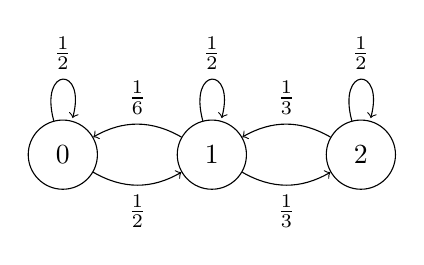
\begin{tikzpicture}
      	\node[state] (0) {0};
      	\node[state] (1)[right=of 0] {1};
      	\node[state] (2)[right=of 1] {2};

      	\path[->]
      	(0) edge [loop above] node {$\frac{1}{2}$} (0)
      	    edge [bend right] node[below] {$\frac{1}{2}$} (1)
      	(1) edge [loop above] node {$\frac{1}{2}$} (1)
      	    edge [bend right] node[above] {$\frac{1}{6}$} (0)
      	    edge [bend right] node[below] {$\frac{1}{3}$} (2)
      	(2) edge [loop above] node {$\frac{1}{2}$} (2)
      	    edge [bend right] node[above] {$\frac{1}{3}$} (1);
      \end{tikzpicture}
    \end{center}
  \end{proposition}

  \begin{definition}{Invariant Distribution}
    Let $\pmb\mu(t)$ denote the probability distribution of random variable $X$ (i,e, $\mu_x(t)=\prob(X_t=x)$). Then
    \[\begin{array}{rrcl}
      &\pmb\mu(t+1)&=&\prob(X_{t+1}=y)=\sum_{x\in S}\prob(X_t=x,X_{t+1}=y)=\sum_{x\in S}\mu_x(t)p_{xy}=\pmb\mu(t)P\\
      \implies&\pmb\mu(t+1)&=&\pmb\mu(t)P
    \end{array}\]
    A distribution $\pmb\pi$ on the state space is called an \textit{Invariant Distribution} if $\pmb\pi=\pmb\pi P$. If $X_t$ has distribution $\pmb\pi$ so will $X_{t+1},\dots$. Every markov chain with a \textit{finite} state space $S$ has an \textit{invariant distribution}. (Not necessarily true if $S$ is infinite).
  \end{definition}

  \begin{proposition}{Finding an Invariant Distribution}
    If an \textit{Invariant Distribution} it is easy to find by solving $\pmb\pi P=\pmb\pi$ and using normalising constant $\sum_{x\in S}\pi_x=1$.
  \end{proposition}

  \begin{remark}{If a Markov chain is irreducible, its invariant distribution (if one exists) is unique}
    If a \textit{Markov Chain} is irreducible and has a finite state space, then it has a unique invariant distribution.
  \end{remark}

  \begin{example}{Markov Chains}
    \begin{itemize}
      \item The \textit{Asymmetric Simple Random Walk} on $\ints$ is $\underbrace{\text{irreducible}}_\text{obvious},\ \underbrace{\text{transient}}_\text{not obvious}$ and has no invariant distribution.
      \item The \textit{Symmetric Simple Random Walk} on $\ints$ is $\underbrace{\text{irreducible}}_\text{obvious},\ \underbrace{\text{recurrent}}_\text{not obvious}$ and has no invariant distribution.
    \end{itemize}
  \end{example}

  \begin{theorem}{Ergodic Theorem for Markov Chains}
    Let $\{X_t\}_{t\in\nats}$ be an irreducible markov chain on state space $S$ (not necessarily finite) with unique invariant distribution $\pmb\pi$. Then
    \[ \forall\ x\in S\quad\lim_{t\to\infty}\frac1t\sum_{s=1}^t \indexed(X_s=x)=\pi_x\]
    i.e. The fraction of time spend in state $x\in S$ tends to $\pi_x$ in the long run.
  \end{theorem}

  \begin{definition}{Period}
    The \textit{Period} of a state $x\in S$ is the greatest common divisor of all possible return times to $x$
    \[ \text{Period}(x):=\text{gcd}\big(\{t>0:\prob(X_t=x|X_0=x)>0\}\big) \]
    \par A state $x\in S$ is \textit{Aperiodic} if $\text{Period}(x)=1$. An irreducible markov chain is \textit{aperiodic} if all its states are aperiodic.
    \par All states in a \textit{communicating class} have the same period.
  \end{definition}

  \begin{proposition}{Marginal Distribution of Irreducible, Aperiodic Markov Chain}
    If an irreducible, aperiodic Markov Chain has an invariant distribution $\pmb\pi$, then
    \[ \forall\ x\in S\quad\mu_x(t)\overset{t\to\infty}{\longrightarrow}\pi_x \]
  \end{proposition}

  \begin{definition}{Reversibility}
    A markov chain $\{X_t\}_{t\in\ints}$ is \textit{Reversible} if all joint distributions are the same forwards and backwards in time. (i.e. the distribution of the chain is the same if it was reversed).
    \par An irreducible markov chain $\{X_t\}_{t\in\ints}$ with transition matrix $P$ is reversible iff
    \[\exists\ \pmb\pi\quad\text{st}\quad\pi_xp_{xy}=\pi_yp_{yx}\ \forall\ x,y\in S\]
    This is the \textit{Local/Detailed Balance Equation}. Note that this is a system of ${|S|\choose2}$ equations which need to be consistent for reversibility to exist.
  \end{definition}

\subsubsection{Continuous Time Markov Process}

  \begin{definition}{Continuous Time Markov Process}
    A stochastic process $\{X_t\}_{t\in\reals}$ is a \textit{Continuous Time Markov Process} on state space $s$ if
    \[ \forall\ s<t\ \&\ x,y\in S\quad\prob(X_t=y|X_s=x,X_u,u\leq s)=\prob(X_t=y|X_s=x) \]
    ie future values only depend on the present value and not past.
    \par If $\forall\ t,s,x,y\ \prob(X_t=y|X_s=x)$ depends only on $x,y,t-s$ (observed values \& change in time) then the process is \textit{Time-Homogeneous}.
    \par For \textit{Time-Homogenous Markov Processes} we let $P(t)$ denote the stochastic matrix with the probability of each possible transition after $t$ time $[P(t)]_{xy}=\prob(X_t=y|X_0=x)$.
  \end{definition}

  \begin{remark}{A \textit{Time-Homogenous Markov Process} is completely described by its initial condition and the family of transition probability matrices $\{P(t):t\geq0$}
    This set of matrices $\{P(t):t\geq0$ is uncountably large.
  \end{remark}

  \begin{definition}{Chapman-Kolmogorov Equations}
    For a \textit{Time-Homogeneous Markov Process} the family of stochastic matrices $\{P(t):t\geq0$ satisfy the following:
    \begin{enumerate}
      \item $P(0)=I$;
      \item $P(t+s)=P(t)P(s)=P(s)P(t)$
    \end{enumerate}
    Hence
    \[ \frac{d}{dt}P(t):=\lim_{\delta\to0}\frac{P(t+\delta)-P(t)}\delta=\lim_{\delta\to0}\frac{\overbrace{P(t)P(\delta)}^\text{ii)}-P(t)}\delta=P(t)\lim_{\delta\to0}\frac{(P(\delta)-I)}\delta \]
    Suppose that $Q:=\displaystyle\lim_{\delta\to0}\frac{P(\delta)-P(0)}\delta=\lim_{\delta\to0}\frac{P(\delta)-\overbrace{I}^\text{i)}}\delta$ exists.\\
    Then $P(t)$ solve the following differential equations, known as the \textit{Chapman-Kolmogorov Equations}
    \[ \frac{d}{dt}P(t)=\underbrace{P(t)Q}_\text{forward eqn.}=\underbrace{QP(t)}_\text{backward eqn.} \]
    The solution to these equations is
    \[ P(t)=P(0)e^{Qt}=e^{Qt}P(0)=e^{Qt}I=e^{Qt} \]
    N.B. $Q$ is called the \textit{Rate Matrix} or \textit{Infinesimal Generator} of the markov process.
  \end{definition}

  \begin{proposition}{Properties of the \textit{Rate Matrix}, $Q$}
    Let $Q$ be the rate matrix of a \textit{continuous-time markov process}. $Q$ has the following properties
    \begin{itemize}
      \item If $n\neq y$ then $\displaystyle q_{xy}:=\lim_{\delta\to0}\frac{[P(\delta)]_{xy}-0}\delta\geq0$. (The off-diagonal elements are non-negative).
      \item $\displaystyle\forall\ x\in S,\ \sum_{y\in S}q_{xy}=\lim_{\delta\to0}\frac{1-1}\delta=0$. The rows of $Q$ sum to 0.
      \item Thus, the diagonal entries $q_{xx}$ are negative. (We denote $-q_{xx}$ by $q_x$)
    \end{itemize}
  \end{proposition}

  \begin{proposition}{Interpreting the \textit{Rate Matrix} $Q$}
    Let $Q$ be the rate matrix of a \textit{continuous-time markov process}.
    \par If the markov process enters state $x$ at time $t$, it will remain in $x$ for a random time which is distributed $\text{Exp}(q_x)$. (Note that $q_x:=-q_xx$).
    \par It the jumps to state $y$ with probability   $\frac{q_xy}{q_x}$, independent of the past.
  \end{proposition}

  \begin{definition}{Invariant Distributions}
    Suppose a \textit{Continuous-Time Markov Process} starts with distribution $\pmb\mu(0)$ on state space $S$ (i.e. $\prob(X_0=x)=[\pmb\mu(0)]_x$). Then, the distribution of $X_t$ is $\pmb\mu(t):=\pmb\mu(0)P(t)=\pmb\mu(0)\underbrace{e^{Qt}}_\text{\tiny CK Eqns}$.
    \par If there exists a distribution $\pmb\pi$ on the state space $S$ st $\forall\ t\geq0\ \pmb\pi=\pmb\pi P(t)=\pmb\pi \underbrace{e^{Qt}}_\text{\tiny CK Eqns}$, then $\pmb\pi$ is an \textit{Invariant Distribution}. This distribution is invariant wrt time.
    \par If a markov process has a finite state space then it definitely has an invariant distribution.
    \par \textit{Invariant Distributions} are not guaranteed to be unique.
  \end{definition}

  \begin{proposition}{Finding an Invariant Distribution}
    Starting with $\pmb\pi=\pmb\pi e^{Qt}$ we find that differentiating wrt $t$ and then evaluating at time $t=0$ we get $\pmb0=\pmb\pi Q$ (The Global Balance Equations). This system of equations can be solved to find an \textit{Invariant Distribution}.
    \par A markov process is \textit{reversible} iff there exists a distribution $\pmb\pi$ on $S$ which satisfies $\pmb\pi_xq_{xy}=\pmb\pi_yq_{yx}\ \forall\ x,y\in S$ (Local balance equations). Solving this system of equations will also find an \textit{Invariant Distribution} but it is not guaranteed to have a solution.
  \end{proposition}

  \begin{theorem}{Ergodic Theorem}
    Let $[X_t]_{t\in\reals^+}$ is an \textit{Irreducible Markov Process} on a state space $S$ and has an invariant distribution $\pmb\pi$. Then
    \[ \forall\ x\in S\quad\pi_x=\lim_{t\to\infty}\frac1t\int_0^t\indexed(X_s=x)ds \]
    Moreover, for an arbitrary initial distribution $\pmb\mu(0)$, $\pmb\mu(t)$ converges to $\pmb\pi$ pointwise (i.e. $\mu_x(t)\overset{t\to\infty}\longrightarrow\pi_x$)
  \end{theorem}

\subsubsection{Poisson Process}

  \begin{definition}{Counting Process}
    A \textit{Counting Process} is a stochastic process $\{N(t)\}_{t\in\reals}$ st
    \begin{enumerate}
      \item $N(0)=0$ and $N(t)\in\ints$ for all $t\geq0$; and,
      \item $N(t)$ is a non-decreasing function of $t$.
    \end{enumerate}
  \end{definition}

  \begin{definition}{Independent Increments}
    A \textit{Process} $\{N(t)\}_{t\in\reals^+}$ is said to have \textit{Independent Increments} if $\forall\ s\in(0,t),\quad(N(t)-N(s))$ is independent of $\{N(u):u\in[0,s]\}$.
  \end{definition}

  \begin{definition}{Poisson Process}
    A \textit{Poisson Process} is a \textit{counting process} $\{N(t)\}_{t\in\reals^+}$ which has independent increments and \underline{at least one} of the following equivalence statements are true
    \begin{itemize}
      \item $\forall\ t\in[0,t]\quad(N(t)-N(s))\sim\text{Po}(\lambda(t-s))$.
      \item $\prob(N(t+\delta)-N(t)=1)=\lambda\delta+o(\delta)$ \underline{and}\\
      $\prob(N(t+\delta)-N(t)=0)=1-\lambda\delta+o(\delta)$ \underline{and}\\
      $\prob(N(t+\delta)-N(t)\geq2)=o(\delta)$.
      \item The \underline{times between successive increments} of the process $N(\cdot)$ are iid $\text{Exp}(\lambda)$ random variables.
    \end{itemize}
    The parameter $\lambda\in\reals^{>0}$ is called the \textit{rate} of the poisson process. \textit{Poisson Processes} are continuous time markov chains.
  \end{definition}

  \begin{example}{Poisson Process}
    Counting the number of cars which have passed a given point over time.
  \end{example}

  \begin{proposition}{Properties of Poisson Processes}
    Define $\{N(t)\}_{t\in\reals^+}$ to be a \textit{Poisson Process} with rate $\lambda$. Then the following properties hold
    \begin{enumerate}
      \item The counting process $\{N(\beta t)\}_{t\in\reals^+}$, with $\beta>0$, is a Poisson Process with rate $\beta\lambda$.
      \item If $\{N_1(t)\}_{t\in\reals^+}$ and $\{N_2(t)\}_{t\in\reals^+}$ are independent poisson processes with rates $\lambda_1$ and $\lambda_2$, respectively, then $\{N(t):=N_1(t)+N_2(t)\}_{t\in\reals^+}$ is a poisson process with rate $\lambda:=\lambda_1+\lambda_2$.
      \item Let $X_1,X_2,\dots$ be a sequence of iid $\text{Bern}(p)$ random vairables, independent of $N(\cdot)$. Define $N_1(t):=\sum_{i=1}^{N(t)}X_i$ and $N_2(t):=\sum_{i=1}^{N(t)}(1-X_i)$ (These are called \textit{Bernoulli Thinnings}). These assign increments in $N(\cdot)$ randomly to either $N_1$ or $N_2$ (with probability $p$).\\
      Then, $N_1(\cdot)$ and $N_2(\cdot)$ are independent poisson processes with rates $\lambda p$ and $\lambda(1-p)$, respectively.
    \end{enumerate}
  \end{proposition}

\subsection{Transformation of Random Variables}

  \begin{example}{Discrete Case}
    Consider rolling a fair die where $\Omega:=\{1,2,3,4,5,6\}$ and $\forall\ \omega\in\Omega\quad\prob(\omega)=\frac16$.
    \par Let $X(\omega)=\omega\ \forall\ \omega\in\Omega$ so the pmf of $X$ is given by
    \[ p_X(i)=\frac16\ \forall\ i\in\{1,\dots,6\} \]
    \par Consider $Y:=X^2$. The pmf of $Y$ is straightforward to work out as each value of $X$ maps to a unique value of $Y$
    \[ P_Y(i)=\frac16\text{ for }\sqrt{i}\in\{1,\dots,6\} \]
    \par Consider $Z:=(X-2)^2$. This is not quite so simple as multiple values of $X$ map to the same value of $Z$.
    \[ p_Z(1)=\frac26;\quad p_Z(i)=\frac16\text{ for }i\in\{0,4,9,16\} \]
  \end{example}

  \begin{example}{Continuous Case}
    Let $X\sim\text{Uniform}[0,1]$ and define $Y:=2X$. We have
    \[ f_X(x)=\begin{cases}1&x\in[0,1]\\0&\text{otherwise}\end{cases}\quad F_X(x)=\begin{cases}0&x<0\\x&x\in[0,1]\\1&x>1\end{cases} \]
    Now consider $Y$ the cdf is
    \[ F_Y(y):=\prob(Y\leq y)=\prob(2X\leq y)=\prob\left(X\leq\frac{y}2\right)=F_X\left(\frac{y}2\right) \]
    We then obtain the pdf for $Y$ by differentiation and the chain rule.
    \[f_Y(y)=F_Y'(y)=\underbrace{\frac12F_X'\left(\frac{y}2\right)}_\text{chain rule}=\frac12f_X\left(\frac{y}2\right)=\begin{cases}\frac12&\frac{y}2\in[0,1]\\0&\text{otherwise}\end{cases}  \]
  \end{example}

  \begin{proposition}{Increasing Functions}
    Let $X$ be a random variable and $Y:=g(X)$ where $g:\reals\to\reals$ is a strictly increasing function. Then, $g$ is invertible on its range (denoted $g^{-1}$). Thus the cdfs for $X$ and $Y$ are related as
    \[ F_Y(y)=\underbrace{\prob(g(X)\leq y)=\prob(X\leq g^{-1}(y))}_\text{as $g$ is increasing}=F_X(g^{-1}(y)) \]
    Differentiating this gives us the pdfs
    \[ f_Y(y)=f_X\left(g^{-1}(y)\right)\frac{dg^{-1}(y)}{dy}=\frac{f_X(x)}{g'(x)}\bigg|_{x=g^{-1}(y)} \]
    The probability mass of $X$ in the interval $(x,x+dx)$ gets mapped to the interval $\big(g(x),g(x+dx)\big)$. By \textit{Taylor Expansion} of $g$ we get $g(x+dx)\simeq g(x)+g'(x)dx$
  \end{proposition}

  \begin{proposition}{General Mappings - Single Random Variable}
    % NOTE is this only true for discrete case?
    Let $X$ be a (discrete) random variable and define $Y:=g(x)$ for any $g:\reals\to\reals$ which is differentiable.
    \par There is a contribution $\frac{f_X(x)}{|g'(x)|}$ from each $x$ such that $g(x)=y$. Where $g'(x)$ is positive or negative does not matter, as it only determines where the pre-image of $(y,y+dy)$ is of the form $(x,x+dx)$ or $(x-dx,x)$. Only the relative widths of the intervals matters for the contribution.
    \par By summing the contributions from all solutions of $g(x)=y$ we get
    \[ p_Y(y)=\sum_{x:g(x)=y}\frac{f_X(x)}{|g'(x)|} \]
    This formula is valid so long as the set $\{x:g(x)=y\}$ is countable. If it is not countable, then $Y$ is a continuous RV (or is a mixed random variable)
  \end{proposition}

  \begin{proposition}{General Mappings - Random Vectors}
    Consider the random vector $\X:=(X_1,\dots,X_d)$ with joint density $f_\X$ and define $\mathbf{Y}:=g(\X)$ for any differentiable $g:\reals^d\to\reals^d$.
    \par Let $J_g(\x)$ denote the \textit{Jacobian} of $g$ at $\x$. Then
    \[ f_\mathbf{Y}(\mathbf{y})=\sum_{\x\in\reals^d:g(\x)=\mathbf{y}}\frac{f_\X(\x)}{|\text{det}(J_g(\x))} \]
    Let $\x$ solve $g(\x)=\mathbf{y}$. In a neighbourhood of $\x$, $g$ is approximately a linear function. By \textit{Taylor Expansion}
    \[ g(\x')\simeq f(\x)+J_g(\x)(\x'-\x)=\mathbf{y}+J_g(\x)(\x'-\x) \]
    for $\x'$ in a small enough neighbourhood of $\x$.
  \end{proposition}

\newpage
\setcounter{section}{-1}
\section{Reference}

  \begin{definition}{Stochastic Matrix}
    A matrix is called a \textit{Stochastic matrix} if:
    \begin{enumerate}
      \item All elements are non-negative.
      \item All rows sum to 1.
    \end{enumerate}
  \end{definition}

  \begin{definition}{Convex Function}
    A function $f:\reals\to(\reals\cup\{+\infty\})$ is \textit{Convex} if, $\forall\ x,y\in\reals,\ \alpha\in[0,1]$, we have
    \[ f(\alpha x+(1-\alpha)y)\leq\alpha f(x)+(1-\alpha)f(y) \]
    A smooth function $f$ is convex iff $f$ is twice differentiable and $f''(x)\geq0\ \forall\ x\in\reals$.\\
    Visually, a function is convex if you can draw a line between any two points on the function and the function lies below the line.
    \begin{center}
      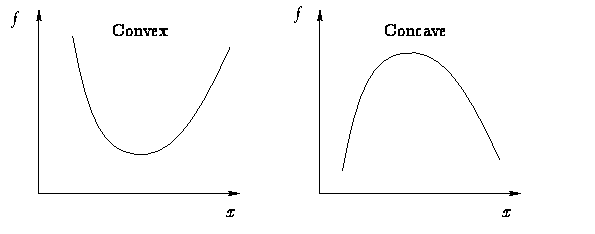
\includegraphics[scale=.5]{convex_concave.png}
    \end{center}
  \end{definition}

  \begin{definition}{Equivalence Relation}
    A relation is an \textit{Equivalence Relation} if it is
    \begin{enumerate}
      \item Reflexive: $i\leftrightarrow i$.
      \item Symmetric: If $i\to j$ then $j\to i$ .
      \item Transitive: If $i\to j$ and $j\to k$ then $i\to k$.
    \end{enumerate}
  \end{definition}

  \begin{definition}{Simple Random Walk}
    A \textit{Simple Random Walk} is a random walk which moves only one step at a time. (i.e. $X_{t+1}=X_t\pm1$). A probability $p$ is defined for $\prob(X_{t+1}=X_t+1)$, this means $1-p$ is the probability of stepping in the other direction. A \textit{Simple Random Walk} is \textit{Assymetric} if $p\neq p-1$.
  \end{definition}

  \begin{definition}{Matrix Exponential, $e^X$}
    Let $X$ be a matrix then we define the \textit{Matrix Exponential} as $e^X:=I+X+\frac{X^2}{2!}+\dots$
  \end{definition}

  \begin{theorem}{Pinsker's Inequality}
    For two distributions $\text{Bern}(p)$ and $\text{Bern}(q)$
    \[ K(q;p)\geq2(q-p)^2 \]
  \end{theorem}

  \begin{definition}{Jacobian Matrix}
    The \textit{Jacobian Matrix} is the first-order partial-derivatives of a multidimensional function $\mathbf{f}:\reals^n\to\reals^m$ wrt each parameter.
    \[ J_f:=\begin{pmatrix}
      \frac{\partial f_1}{\partial x_1}&\frac{\partial f_1}{\partial x_2}&\dots&\frac{\partial f_1}{\partial x_n}\\
      \frac{\partial f_2}{\partial x_1}&\frac{\partial f_2}{\partial x_2}&\dots&\frac{\partial f_2}{\partial x_n}\\
      \vdots&\vdots&\ddots&\vdots\\
      \frac{\partial f_m}{\partial x_1}&\frac{\partial f_m}{\partial x_2}&\dots&\frac{\partial f_m}{\partial x_n}
    \end{pmatrix}\]
  \end{definition}

\subsection{Notation}
  \textit{Multi-Armed Bandit Problem}\\
  \begin{tabular}{|c|l|}
    \hline
    $p_{x,y}$&$\prob(X_{t+1}=x|X_{t}=y)$ for a \textit{time homogenous markov process}.\\
    $I(t)$&Arm played in round $t$.\\
    $N_i(t)$&$\sum_{s=1}^t\identity\{I(s)=i\}$ Number of times arm $i$ was played in first $t$ rounds.\\
    $S_i(t)$&$\sum_{s=1}^tX_i(s)\identity\{I(s)=i\}$ Total reward from arm $i$ in first $t$ rounds.\\
    $\hat\mu_{i,N_i(t)}$&$\frac{S_i(t)}{N_i(t)}$ sample mean reward from arm $i$ in first $t$ rounds.\\
    $\Delta_i$&$\mu^*-\mu_i$ the arm gaps from a $K$-armed bandit.\\
    $X_i(t)$&RV modelling the result if arm $i$ was played on round $t$.\\
    \hline
  \end{tabular}

  \textit{Markov Decision Problems}\\
  \begin{tabular}{|c|l|}
    \hline
    $T$&Time-Horizon.\\
    $S$&State-Space.\\
    $A$&Action-Space.\\
    $A(s)$&Available actions when in system state $s$.\\
    $Y_t$&Random variable modelling action taken by the agent at epoch $t$.\\
    $r_t(s,a)$&The value of the reward received at epoch $t$ if the system is in state $s$ and the agent takes action $a$.\\
    $p_t(s'|s,a)$&The probability that the system is in state $s'$ at time $t+1$ given at time $t$ the system was in state $s$ and the agent took action $a$.\\
    $d_t(\cdot),\ q_t(\cdot)$&The decision function at epoch $t$.\\
    $\pi$&A decision policy.\\
    $HR(T)$&The set of policies on time-horizon $T$ in which the decision rules are HRs.\\
    $MD(T)$&The set of policies on time-horizon $T$ in which the decision rules are MDs.\\
    $\prob^\pi,\ \expect^\pi$&Probability and expectation given policy $\pi$ is being used.\\
    $T^\pi$ & The expected reward for a given policy.\\
    $u*(s)$ & The terminal reward for a given MDP.\\
    \hline
  \end{tabular}

  \textit{General}\\
  \begin{tabular}{|c|l|}
    \hline
    $z_{m:n}$&The $m^{th}$ to the $n^{th}$ elements of a sequence $\{z_t\}$.
    \hline
  \end{tabular}

\subsubsection{Asymptotic Notation}

  \begin{definition}{Oh Notation}
    Let $f,g:\reals^+\to\reals$.
    \par We say $f=o(g)$ (little oh of $g$) at 0 if $\frac{f(x)}{g(x)}\overset{x\to0}\longrightarrow0$.
    \par We say $f=O(g)$ (big oh of $g$) at 0 if $\exists\ c>0$ st $|f(x)|\leq c|g(x)|$ in a neighbourhood of 0.
    \par $f=o(g)$ at infinity and $f=O(g)$ at infinity are defined analogously.
  \end{definition}

  \begin{definition}{Omega Notation}
    Let $f,g:\reals^+\to\reals$.
    \par We say $g=\omega(g)$ if $o(f)$ and we say $f=\Omega(g)$ if $g=O(f)$.
  \end{definition}

  \begin{example}{Oh \& Omega Notation}
    Define $f(x)=x,\ g(x)=\sin(x)$ and $h(x)=x^2$.\\
    Then, $g=O(f)$ at 0 and $g=o(f)$ at infinity. $h=o(f)$ at 0 and $h=\omega(f)$ at infinity.
  \end{example}

\end{document}
